\documentclass[a4paper, twoside, 11pt]{report}

%% Language and font encodings
\usepackage[english]{babel}
\usepackage[utf8x]{inputenc}
\usepackage[LGR,T1]{fontenc}
\usepackage{listings}
\usepackage{lstautogobble}
% \usepackage{newcomputermodern}
\usepackage{selinput}
\usepackage{textalpha}
\usepackage{minted}
\usepackage{caption}
\usepackage{amssymb}
\usepackage[fleqn]{mathtools}
\usepackage[numbers]{natbib}
\usepackage{tikz}
\usepackage{xcolor}
\usepackage{pgfplots}
\usepackage{import}
\usepackage{xspace}
\usepackage{enumerate}
\usepackage{amsmath}
\usepackage{graphicx}
\usepackage[colorinlistoftodos]{todonotes}
\usepackage[colorlinks=true, allcolors=blue]{hyperref}
\usepackage[a4paper,top=3cm,bottom=2cm,left=3cm,right=3cm,marginparwidth=1.75cm]{geometry}
\usepackage{ifthen}
\usepackage{algorithm}
\usepackage{algpseudocode}
\usepackage{algorithmicx}
\usepackage{chngcntr}
\usepackage{tabularx}
\usepackage{lineno}


\usetikzlibrary{
    decorations.pathreplacing,
    arrows,
    shapes,
    shapes.gates.logic.US,
    circuits.logic.US,
    calc,
    automata,
    positioning,
    intersections,
    calligraphy,
    tikzmark
}
\setminted{
    xleftmargin=16pt,
    breakanywhere=true,
    breaklines=true,
    linenos=true,
    autogobble,
}

% colours
\newcommand{\violet}[1]{\textcolor{violet}{#1}}
\newcommand{\blue}[1]{\textcolor{blue}{#1}}
\newcommand{\red}[1]{\textcolor{red}{#1}}
\newcommand{\teal}[1]{\textcolor{teal}{#1}}
\pgfplotsset{compat=1.16}
\raggedbottom
\setcounter{secnumdepth}{4}
\allowdisplaybreaks % allow environments to break

\def\UrlBreaks{\do\/\do-}

% code listing
\lstdefinestyle{main}{
    numberstyle=\tiny,
    breaklines=true,
    showspaces=false,
    showstringspaces=false,
    tabsize=2,
    numbers=left,
    basicstyle=\ttfamily,
    columns=fixed,
    fontadjust=true,
    basewidth=0.5em,
    autogobble,
    xleftmargin=3.0ex,
    mathescape=true
}
\newcommand{\dollar}{\mbox{\textdollar}} %
\lstset{style=main}

\title{Parser Combinators in Languages without User-Defined Operators}
\author{Eugene Lin}

\frenchspacing

\providecommand*{\listingautorefname}{listing}
\providecommand*{\algorithmautorefname}{algorithm}
\newenvironment{capminted}{\captionsetup{type=listing}}{\vspace{\baselineskip}}

\newcommand{\fixtilde}{\raisebox{-0.25em}\textasciitilde}

\newcommand{\mult}{<\fixtilde>\xspace}
\newcommand{\multl}{<\fixtilde\xspace}
\newcommand{\multr}{\fixtilde>\xspace}
\newcommand{\ap}{<*>\xspace}
\newcommand{\apl}{<*\xspace}
\newcommand{\apr}{*>\xspace}
\newcommand{\pa}{<**>\xspace}
\newcommand{\choice}{<|>\xspace}
\newcommand{\fmap}{<\$>\xspace}
\newcommand{\constfmapl}{<\$\xspace}
\newcommand{\constfmapr}{\$>\xspace}
\newcommand{\pamf}{<\&>\xspace}

\newcommand{\tsext}{TypeScript$^*$\xspace}

\newcounter{equi}
\setcounter{equi}{1}
\newcommand{\equi}[1][]{%
    \ifthenelse
        {\equal{#1}{}}%
        {%
            \text{({\sc\roman{equi}})}%
            \stepcounter{equi}%
        }%
        {\text{({\sc\romannumeral#1})}}%
}
% usage: \equi to get and increment, \equi[x] to reference equivalence x

\begin{document}
\counterwithin{listing}{chapter}
\begin{titlepage}

\newcommand{\HRule}{\rule{\linewidth}{0.5mm}} % Defines a new command for the horizontal lines, change thickness here

%----------------------------------------------------------------------------------------
%	LOGO SECTION
%----------------------------------------------------------------------------------------


\includegraphics[width=8cm]{title/logo.eps}\\[1cm] % Include a department/university logo - this will require the graphicx package
 
%----------------------------------------------------------------------------------------

\center % Center everything on the page

%----------------------------------------------------------------------------------------
%	HEADING SECTIONS
%----------------------------------------------------------------------------------------

\textsc{\LARGE MEng Individual Project}\\[0.5cm] % Name of your university/college
\textsc{}\\[1.5cm] % Major heading such as course name
% \textsc{\Large Interim Report}\\[1.5cm] % Major heading such as course name
\textsc{\Large Imperial College London}\\[0.5cm] % Major heading such as course name
\textsc{\large Department of Computing}\\[0.5cm] % Minor heading such as course title

%----------------------------------------------------------------------------------------
%	TITLE SECTION
%----------------------------------------------------------------------------------------
\makeatletter
\HRule \\[0.4cm]
{ \huge \bfseries \@title}\\[0.4cm] % Title of your document
\HRule \\[1.5cm]
 
%----------------------------------------------------------------------------------------
%	AUTHOR SECTION
%----------------------------------------------------------------------------------------

\begin{minipage}{0.4\textwidth}
\begin{flushleft} \large
\emph{Author:}\\
\@author % Your name
\end{flushleft}
\end{minipage}
~
\begin{minipage}{0.4\textwidth}
\begin{flushright} \large
\emph{Supervisor:} \\
Jamie Willis \\[1.2em] % Supervisor's Name
\emph{Second Marker:} \\
Dr. Peter McBrien % second marker's name

\end{flushright}
\end{minipage}\\[2cm]
\makeatother

% If you don't want a supervisor, uncomment the two lines below and remove the section above
%\Large \emph{Author:}\\
%John \textsc{Smith}\\[3cm] % Your name

%----------------------------------------------------------------------------------------
%	DATE SECTION
%----------------------------------------------------------------------------------------

{\large \today}\\[2cm] % Date, change the \today to a set date if you want to be precise

\vfill % Fill the rest of the page with whitespace

\end{titlepage}

\newcounter{abstractpage}
\setcounter{abstractpage}{\value{page}}

\begin{abstract}
    \thispagestyle{plain}
    \setcounter{page}{\value{abstractpage}}

    Parser combinators often embody the principles of software engineering best practices, from abstraction to simplicity.
    They provide an effective solution to the problem of parsing, offering numerous benefits such as the ability for the user to define functionality in the host language, to creating parsers that closely resemble the original grammar.
    However, there can be a high barrier to entry: not only can the idea of functional programming seem daunting to some, but pitfalls such as left-recursion can often serve to complicate an otherwise intuitive experience.
    Many existing solutions for left-recursion remain highly theoretical or incomplete, thus preventing real usage.

    This project remediates some of these hurdles by creating a lightweight parser combinator library in TypeScript as well as a preprocessing pipeline to support additions, such as custom operators, to TypeScript.
    Furthermore, the preprocessor can also perform static analysis over the structure of the program, providing an opportunity to optimise parsers.
    A key contribution of this project lies in this analysis: pitfalls such as left-recursion can be detected and automatically corrected, while maintaining the desired semantics, via a series of transformation and reduction steps.

    \setcounter{abstractpage}{\value{page}}
\end{abstract}

\setcounter{page}{\value{abstractpage}}
\stepcounter{page}
\setcounter{abstractpage}{\value{page}}

\renewcommand{\abstractname}{Acknowledgements}
\begin{abstract}
    \thispagestyle{plain}
    \setcounter{page}{\value{abstractpage}}

    First and foremost, I need to extend an immense deal of gratitude to Jamie.
    Not only would this project have been impossible without his support and guidance, I would not have even been introduced to the idea of parser combinators in the first place.
    I would also like to extend my gratitude to those who took the time to proofread this entire report on \emph{extremely} short notice.

    Next, I would like to thank the friends I have made at university; the past four years would not have been the same without you all.
    And for my friends from before university; I cannot thank you all enough for your patience with me.
    Finally: I want to thank my family, especially my parents, for all the support they have given me.

    \setcounter{abstractpage}{\value{page}}
\end{abstract}

\setcounter{page}{\value{abstractpage}}
\stepcounter{page}

\tableofcontents

\chapter{Introduction}
\label{chap:intro}

With the exception of hand-crafted parsers, most parsers can be placed into one of two categories; parser combinators, such as \textit{Parsley} \cite{willis18} and \textit{megaparsec} \cite{megaparsec}, and parser generators, including \textit{Yacc} \cite{johnson75} and \textit{ANTLR} \cite{parr14}.
One major difference lies in how the user specifies the language; the former (parser \textbf{generators}) requires a preprocessing step over a DSL (domain-specific language) representing the grammar in a form resembling EBNF (extended Backus-Naur form).
This generates source code in the host language, which can then be used to parse input.

On the other hand, parser \textbf{combinators} are implemented directly in the host language and do not require a preprocessing stage.
Simple functions, which are individual parsers, take in an input and either give a successful (which would contain the parsed tree) or a failed response.
These can be combined in a number of ways to produce more complex parsers of arbitrary types.

As expected, both approaches come with their respective benefits and drawbacks.
A major disadvantage of parser generators is the generated parse tree; this is typically in a form specified by the creators of the library and may be tedious to traverse in order to convert into a desired structure, whereas a parser combinator can directly generate the desired tree in the host language.
An advantage of parser generators is the ability to specify precedence rules, whereas this may have to be done by nesting the grammar with some parser combinator libraries.
However, libraries often provide this functionality on top of the base combinators.

Another major advantage for parser combinators is the ability to abstract common patterns in the host language.
For example, the aforementioned precedence rules could trivially be implemented by the user when using parser combinators.
This advantage can be seen in \autoref{fig:gen_vs_comb}.
In this example, a common pattern of a comma separated list is abstracted out by a user-defined function \texttt{commaSep}.
Not only is the representation simpler, it also provides the desired structure of a list of elements (rather than two parse trees that have the same shape) and has less repetition.

\begin{figure}[H]
    \centering
    \begin{minipage}{0.33\textwidth}
        \begin{minted}{antlr}
            arr : '[' es ']' ;
            es  : e | e ',' es ;
            obj : '{' ps '}' ;
            ps  : p | p ',' ps ;
        \end{minted}
    \end{minipage}
    \hfill
    $\leadsto$
    \hfill
    \begin{minipage}{0.56\textwidth}
        \begin{minted}{scala}
            def commaSep[A](p: P[A]): P[List[A]]
              = p <::> many(',' *> p)
            val arr = '[' *> commaSep(e) <* ']'
            val obj = '{' *> commaSep(p) <* '}'
        \end{minted}
    \end{minipage}
    \caption{Left: example grammar (\textit{ANTLR4}) for defining array and object literals, right: representation of the same grammar with parser combinators (\textit{Parsley})}
    \label{fig:gen_vs_comb}
\end{figure}

With parser combinators, or more generally recursive descent parsers, a key limitation is the inability to handle left-recursive grammars.
A fairly mechanical technique to overcome this is to simply eliminate the left-recursive production (in general, a non-terminal production $A \to A\alpha\ |\ \beta$ can be written as $A \to \beta R$ and $R \to \alpha R\ |\ \epsilon$ \cite{dragon}).
This can be seen in \autoref{fig:orig_vs_rewrite}.
While this can be quite easily performed with a simple grammar, it already begins to look less intuitive than the original production, and one could imagine the complexity that would arise from more complex grammars.

\begin{figure}[H]
    \centering
    \begin{minipage}{0.375\textwidth}
        \begin{lstlisting}[numbers=none, xleftmargin=0pt]
            expr ::= expr '+' nat | nat
        \end{lstlisting}
    \end{minipage}
    \hfill
    $\leadsto$
    \hfill
    \begin{minipage}{0.375\textwidth}
        \begin{lstlisting}[numbers=none, xleftmargin=0pt]
            expr  ::= nat exprR
            exprR ::= '+' nat exprR | $\epsilon$
        \end{lstlisting}
    \end{minipage}
    \caption{Left: original grammar for adding numbers, right: rewritten grammar (without left recursion)}
    \label{fig:orig_vs_rewrite}
\end{figure}

The aim of this project is to lower the barrier to entry for using parser combinators.
The first of which is the host language - the vast majority of existing libraries are built in functional languages for obvious reasons, including the functional nature of this style of parsing.
However, this adds an additional burden on the user in that they may have to learn an entirely new paradigm.
As such, this project introduces a parser combinator library built entirely in TypeScript: \textit{Teaspoon}\footnote{A fitting name for files with an extension of \texttt{.tsp}}.
Another barrier to entry is the small nuances that exist \cite{willis21}, such as the previously stated limitations with left-recursive productions.

This project contributes a preprocessor over TypeScript that not only allows for the use of combinators as operators, rather than functions, but also perform analysis over the combinators in order to aid the user and remediate detected anti-patterns.
The use of a preprocessor also allows for the definition of operators beyond what the language natively provides, thus permitting syntax which can be more intuitively read (compared to numerous nested function calls) such as:

\begin{minted}{teaspoon_lex.py:TeaspoonLexer -x}
    let u = chr('_');                      // underscore
    let l = re(/[A-Za-z]/);                // letter
    let d = re(/[0-9]/);                   // digit
    let c = (xs: string[]) => xs.join(""); // concatenate

    let id_op = c <$> ((u <|> l) <:> many(u <|> l <|> d));
    let id_fn =
      fmap(c, liftCons(choice(u, l), many(choice(choice(u, l), d))));
\end{minted}

\paragraph*{Outline}
This report begins by exploring parser combinators (and parsers in general) in detail, alongside the common pitfalls that may arise from their use in \autoref{chap:background}.
With this intuition on how parsing can be performed by building up smaller parsers, \autoref{chap:library} highlights the design decisions and underlying implementation of the TypeScript-based parser combinator library.
While the library is functional on its own, a preprocessor is required to support custom operators.
This is explored in \autoref{chap:preprocessor}, which details the architecture of the preprocessor, the design decisions made, as well as the extensions made to TypeScript.
The optimisations found in the preprocessor are analysed in greater detail in \autoref{chap:oaa}, with \autoref{chap:soundness} verifying the soundness of the transformations performed.
The efficacy of these optimisations are then evaluated in \autoref{chap:evaluation} alongside the performance of the library in different scenarios.
Finally, \autoref{chap:conclusion} details the contributions made, as well as how this work can be explored further.

\chapter{Background}
\label{chap:background}

\section{Parsers}
\label{sec:parsers}

A parser forms the first stage of the compilation pipeline.
Intuitively, parsing (also referred to as syntactic analysis) is the process of obtaining meaning from an input, typically a string, and deriving meaning in some form of structure, based on some grammar.
For example, consider a simple expression: within these operators there are a series of precedence rules that should be adhered to, rules that are intuitively known.
However, this needs to be formally specified to a parser in order to generate the parse tree in \autoref{fig:tree}; the original input string has no real meaning without a structure.
\begin{figure}[H]
\centering
\begin{tikzpicture}
    \node[anchor=east] at (0, 0) {\texttt{-1+2*(3-4)}};
    \node at (1.4, 0) {$\leadsto$};
    \begin{scope}[shift={(4, 1.5)}]
        \node (o) at (0, 0) {\texttt{+}};
        \node (ol) at (-1, -1) {\texttt{-}};
        \node (or) at (1, -1) {\texttt{*}};
        \node (olc) at (-1, -2) {\texttt{1}};
        \node (orl) at (0.5, -2) {\texttt{2}};
        \node (orr) at (1.5, -2) {\texttt{-}};
        \node (orrl) at (1, -3) {\texttt{3}};
        \node (orrr) at (2, -3) {\texttt{4}};

        \draw
        (o) -- (ol)
        (o) -- (or)
        (ol) -- (olc)
        (or) -- (orl)
        (or) -- (orr)
        (orr) -- (orrl)
        (orr) -- (orrr);
    \end{scope}
\end{tikzpicture}
\caption{An example parse tree for a simple expression}
\label{fig:tree}
\end{figure}

It is important to first differentiate between the types of parsers.
In general, parsers can be split into two categories; top-down (including $\text{LL}(k)$ parsers, recursive descent) and bottom-up (including $\text{LR}(k)$ parsers, shift-reduce).
The former builds the AST from the root nodes to the leaf nodes, whereas the latter builds from the leaf nodes to the root nodes (hence bottom-up).

Top-down parsing begins with a non-terminal, and once a token is identified, it is used to `fill' in the tree, creating a root node and child nodes based on the expected structure of the root node from the first identified token.
At this point, any non-terminals that are in the tree are produced in the same way, building from the root node downwards.
Due to the recursive nature of this style of parsing, it is evident that recursively applying a rule can be problematic if care is not taken, as discussed in \autoref{ssec:lrec}.

On the other hand, bottom-up parsing tries to use all the rules (whereas top-down tries to match a non-terminal by trying each of the rules), and replaces it with a non-terminal, by using the production in reverse.
Bottom-up parsing succeeds when the whole input is replaced by the start symbol.

Both $\text{LL}(k)$ and $\text{LR}(k)$ parsers perform left-to-right scanning and have $k$ tokens of look-ahead \cite{dragon}, but differs in the former having left-most derivation whereas the latter has right-most derivation.
Note that $\text{LL}(n) \subseteq \text{LR}(n)$, hence $\text{LR}$ parsers are more powerful.

\section{Types}
\label{sec:type}

Throughout this section, the type \texttt{Parser} will be used.
In TypeScript, the host language for the project, this is defined as the following (where \texttt{Result} captures whether input is consumed, as well as whether the parser succeeded).

\begin{minted}{typescript}
type Parser<A> = (s: State) => Result<A>;
\end{minted}

However, for brevity and readability, Haskell's type syntax will be used instead.
Note that TypeScript does not have a specific type for characters, as such any use of \texttt{Char} in Haskell would be a use of \text{string} in TypeScript (however, a fixed length of 1 is assumed).
Note that additional work will also be required to concatenate a list of singleton strings into a single string, which will likely lead to the produced code being more verbose.

\subsection{Primitives}
\label{ssec:primitives}

As combinator parsing involves joining together basic primitives, it is natural to begin with the most basic parsers, as described by Hutton \& Meijer (1999) \cite{hutton99}.
The first primitive is that of a parser that will always succeed if it is able to consume input and fail otherwise.
This has the signature \texttt{item :: Parser Char}.

On the other hand, a parser that always fails, regardless of the input, is also required.
Note that this comes from the \texttt{Alternative} typeclass.
This parser can be referred to as \texttt{empty :: Parser a} - the type of which is irrelevant as no parse tree will be produced.

Finally, a primitive that lifts a pure value into the context of a parser is also required.
Note that this is in both the \texttt{Applicative} and \texttt{Monad} typeclasses, referred to as \texttt{pure} and \texttt{return} respectively.
As \texttt{Applicative} is a superclass of \texttt{Monad}, by default \texttt{return} refers to \texttt{pure}.
This has the following signature:

\begin{minted}{haskell}
return :: a -> Parser a
\end{minted}

Alongside \texttt{(>{}>=)} in \autoref{ssec:monad}, this can be used to form the parser \texttt{satisfy}, which parses a character based on a predicate.

While it is possible to define \texttt{satisfy} in terms of \texttt{item}, via the use of \texttt{bind}, it is also possible to go in the `opposite' direction by defining \texttt{item} as \texttt{satisfy (const true)}.
Using \texttt{satisfy} as the primitive is often preferable when compared to using \texttt{item} as \texttt{bind} significantly decreases the efficacy of inspection.
This primitive comes from a natural interpretation of reading a character and has the type:

\begin{minted}{haskell}
satisfy :: (Char -> Bool) -> Parser Char
\end{minted}

\subsection{Functor}
\label{ssec:functor}

A functor is a typeclass that allows for a function to be applied to the contained pure value, without altering the overall structure \cite{allen2016haskell}.
This is done with the following function:

\begin{minted}{haskell}
fmap :: (a -> b) -> Parser a -> Parser b
\end{minted}

It can also be written as \texttt{(<\$>)}, for infix notation.

By giving parsers this property, the user is now able to modify the resulting parse tree without changing any other properties of the parse result.
This includes the success of the result: if it was a failure, then nothing is done.
A concrete use of this is to create a parser for natural numbers: after consuming a sequence of characters (hence forming a string), it can be converted into an integer, giving a \texttt{Parser Int}.

Using the above, a derived combinator \texttt{(<\$)} arises.
The first argument is used in place of the resulting parse tree from the second argument (a \texttt{Parser}), if the parse was successful.
This has the signature:

\begin{minted}{haskell}
(<$) :: a -> Parser b -> Parser a
x <$ p = const x <$> p
\end{minted}

By treating \texttt{Parser}s as \texttt{Functor}s, it is possible to assign meaning to a result, by transforming it beyond that of a literal string.

\subsection{Applicative}
\label{ssec:applicative}

First note that an alternative typeclass to this is \texttt{Monoidal}, where both can capture the idea of sequencing parsers.
Earlier references, such as Wadler (1985) \cite{wadler85} and Fokker (1995) \cite{fokker95}, provide sequencing in the form of pairs:

\begin{minted}{haskell}
(<~>) :: Parser a -> Parser b -> Parser (a, b)
\end{minted}

While this may seem intuitive for simple combinations of parsers, it can become tedious and difficult to handle when more parsers are sequenced together.
For example, consider sequencing three parsers, leading to nested pairs:

\begin{minted}{haskell}
pa   :: Parser a
pb   :: Parser b
pc   :: Parser c
pabc :: Parser ((a, b), c)
  = pa <~> pb <~> pc
\end{minted}

In general use cases, the use of pairs to represent sequential operation can become too restrictive.
Naturally, this leads to a more general form.

Note that \texttt{Applicative}s allow for sequencing of functional computations but do not allow for the use of results from earlier computations (which are provided with \texttt{Monad} in \autoref{ssec:monad}).
They also do not generally enforce an execution order (however in the context of \texttt{Parser}s, this is enforced by \texttt{Monad}).
Recall the \texttt{return} `primitive' mentioned earlier in \autoref{ssec:primitives}, in the \texttt{Applicative} context, this is referred to as \texttt{pure}, however the semantics remain the same.
The method \texttt{(<*>)} can be intuitively thought of as a more general function application \cite{hutton16} in the context of \texttt{Parser}s:

\begin{minted}{haskell}
(<*>) :: Parser (a -> b) -> Parser a -> Parser b
\end{minted}

The aforementioned example of \texttt{(\mult)} can be written as follows (in terms of \texttt{<*>}) - note that the first parser is mapped into a parser of a function:

\begin{minted}{haskell}
px <~> py = (,) <$> px <*> py
\end{minted}

Important derived combinators that arise from this include the following \cite{yoda}:

\begin{minted}{haskell}
(<*)   :: Parser a -> Parser b -> Parser a
p <* q = const <$> p <*> q

(*>)   :: Parser a -> Parser b -> Parser b
p *> q = flip const <$> p <*> q

(<**>) :: Parser a -> Parser (a -> b) -> Parser b
p <**> q = (flip ($)) <$> p <*> q

(<:>)  :: Parser a -> Parser [a] -> Parser [a]
p <:> ps = (:) <$> p <*> ps
\end{minted}

The first two combinators execute both parsers, and only results in a successful parse when both succeed.
However, only one of the two parsed results are used, and the other is discarded.
The next combinator (\texttt{<**>}, or `reverse ap') is similar to the original \texttt{<*>}, but instead has the function as the second parser.
Finally, the \texttt{<:>} combinator, also referred to as lifted cons, allows joining an element to a list of elements in the \texttt{Parser} context.

In addition to these derived combinators, it is also possible to define `lift's, which combine $n$ parsers using a function.
Note that the derived combinators can also be defined in terms of lifts.
For example, \texttt{<:>} and \texttt{<**>} can be defined as the following (in TypeScript), where the first parameter is an uncurried function that contains the desired functionality:

\begin{minted}{typescript}
  let lift_cons = lift2((p: A, ps: A[]) => [p, ...ps], p, ps);
  let rev_ap    = lift2((p: A, q: (a: A) => B) => q(p), p, q);
\end{minted}

With these combinators, it is now possible to parse combinations of primitives, given a completely fixed structure.

\subsection{Alternative}
\label{ssec:alternative}
Note that \texttt{Alternative} exists as a subclass of \texttt{Applicative}, additionally it is closely related to \texttt{MonadPlus}, where the zero elements are \texttt{empty} and \texttt{mzero} respectively, and the combining functions are \texttt{(<|>)} and \texttt{mplus}.
For simplicity, only the \texttt{Alternative} definitions are included.

The \texttt{empty} parser has been previously mentioned in \autoref{ssec:primitives}, as a primitive parser.
Note that combining any parser with the \texttt{empty} parser by using the combining function will result in the original parser.
This has the signature:

\begin{minted}{haskell}
(<|>) :: Parser a -> Parser a -> Parser a
\end{minted}

This combinator captures the ability to choose between alternatives.
For example, the parser \texttt{x <|> y} will first attempt to parse \texttt{x}, however if it fails, it will then attempt to parse \texttt{y}.
Note that with the \textit{Parsec} \cite{leijen01} family of parsers, the second parser is only attempted when the first parser does not consume input.
However, this behaviour may not be desired thus a parser may want to roll back any consumption, or `backtrack'.
Backtracking is done with \texttt{try} (in the case of \textit{Parsec}), where the parser acts as if it did not consume input on a failure.
If both fail, the overall parser fails, however if either succeed, the first to succeed is the result of the parser.
It is crucial to note that while \texttt{\choice} is associative, it is not commutative.

Alternatives, including \texttt{empty}, provide a number of laws that can be beneficial for performing optimisations.
Note that these laws are not always general, but hold for parsers.
These include the left and right neutral laws $(1, 2)$, as well as the left absorption law $(3)$ and left catch law $(4)$:
\begin{align*}
    \texttt{empty \choice p} & \Rightarrow \texttt{p} & (1) \\
    \texttt{p \choice empty} & \Rightarrow \texttt{p} & (2) \\
    \texttt{empty \ap p} & \Rightarrow \texttt{empty} & (3) \\
    \texttt{pure x \choice p} & \Rightarrow \texttt{pure x} & (4)
\end{align*}

The left absorption (zero) law is generally accepted, whereas the right absorption law is not.
In parsers, the parser \texttt{p} in \texttt{p \ap empty} may consume input, thus changing the state.
The left catch law essentially states that \texttt{pure} (from \texttt{Applicative}s) represents a successful parse (specifically in the context of parsers).

\bigskip

By using the \texttt{Alternative} typeclass, the parsers are able to capture choice.
Additionally, this allows for further combinators such as \texttt{many} to be defined, where sequences of arbitrary length can be generated; without choice, a production would either be a fixed finite number, or an infinite length.
For example:

\begin{lstlisting}
A ::= 'a' A -- infinitely many 'a's
B ::= 'b' C -- exactly 2 'b's
C ::= 'b'   -- exactly 1 'b'
\end{lstlisting}

However, with choice, it is therefore possible to define the following, where as many \texttt{'a'}s are parsed as possible, until there are no more \texttt{'a'}s to consume (thus terminating the first branch of the parser (\texttt{'a' A})):

\begin{lstlisting}
A ::= 'a' A | $\varepsilon$
\end{lstlisting}

\subsection{Monad}
\label{ssec:monad}

By using the \texttt{Monad} typeclass, the bind operator is introduced.
This has the signature:

\begin{minted}{haskell}
(>>=) :: Parser a -> (a -> Parser b) -> Parser b
\end{minted}

An interpretation of this combinator is similar to that of \texttt{<*>} in \autoref{ssec:applicative}, however the result of the first parser is applied to a function that creates the second parser, rather than being applied to the result of the second parser (which is a function).
However, as the result of the first parser can directly influence the result of the second parser (since the function can use the result of the first parse), this creates a guarantee on the order of operations.
The first parser must be executed before the function that produces the second parser can be.

While this permits for context-sensitive parsing, as the function producing the second parser can access the results of the previous parse, it severely impacts the efficacy of inspection and analysis.
Due to this decrease in efficacy, bind will not be a primary focus for subsequent optimisations, but it is still important to note due to its power (it can implement both \texttt{\ap} and \texttt{\fmap}).

\section{Pitfalls}
\label{sec:pitfalls}

\subsection{Left Recursion}
\label{ssec:lrec}

One of the motivating anti-patterns is the difficulty of handling left-recursion \cite{willis21}.
Recall the basic expression grammar \texttt{expr}, first mentioned in \autoref{chap:intro}.
\begin{lstlisting}
    expr ::= expr '+' nat | nat
\end{lstlisting}
Using the combinators that have been introduced above, this can be written as the following (actually performing the calculations):

\begin{capminted}
    \begin{minted}{teaspoon_lex.py:TeaspoonLexer -x}
        lazy expr = expr <**> ((x => y => x + y) <$ chr('+')) <*> nat <|> nat;
    \end{minted}
    \vspace{-0.5\baselineskip}
    \caption{Running example of simple addition parser}
    \label{lst:running_example}
\end{capminted}

Now consider the execution of this parser: when the parser attempts to parse an \texttt{expr}, the first thing it will do is attempt the first `choice'.
In this choice, it will then attempt to parse the first parser of that sequence - this is the left-most parser, and it is \texttt{expr}.
Naturally, it will then attempt to parse another \texttt{expr}; however, at this point no input has been consumed, and the input state remains unchanged - the parser is back where it started; it has looped and made no progress.

The example above shows direct left-recursion, where the production is the left-most lexeme in its own rule.
In general, left-recursion can be classified into one of three categories; \textbf{direct}, \textbf{indirect}, and \textbf{hidden} \cite{diflrecs}.
A simple example of an indirect left-recursion would exist in the following grammar, where $A$ is not directly in the right-hand side of the rule for $A$, but exists a level down, in the rule for $B$.
Note that $A$ and $B$ are non-terminals and $\alpha$ and $\beta$ are terminals.
\begin{align*}
    A & \rightarrow B \alpha\ |\ \cdots \\
    B & \rightarrow A \beta\ |\ \cdots
\end{align*}
Finally, hidden left-recursion occurs when the first non-empty lexeme is itself.
For example, this can be seen in the production $A \rightarrow \epsilon A$, where $\epsilon$ is empty.
The example given for hidden left-recursion is very simple, however it can also be indirect; for example $A \rightarrow BA$, and $B \rightarrow^* \epsilon$ (where $\rightarrow^*$ means $B$ eventually reduces to $\epsilon$) is also left-recursive.
Note that even $\text{LR}(k)$ parsers are unable to handle hidden left-recursion, as mentioned by Nederhof \& Sarbo (1993) \cite{nederhof93}.

\subsection{`Dangling Else'}
\label{ssec:dangling_else}

A common pitfall that could be encountered is the parsing of keywords in many programming languages.
For example, if the production rules for keywords in a language consisted of $\ \cdots\ |\ \texttt{'in'}\ |\ \texttt{'include'}\ |\ \cdots$ there may be a number of issues.
The first of which is the order in which the rules are tested in.
As \texttt{Alternative} will attempt the rules from left-to-right (as mentioned in \autoref{ssec:alternative}), once it matches \texttt{'in'}, it will have parsed a keyword, with the remainder being \texttt{'clude'}, rather than parsing the longest string.
As such, some care will need to be taken when constructing rules for possible ambiguity.

Another pitfall may arise without the use of \texttt{attempt}.
For example, if the grammar were to be rewritten as $\ \cdots\ |\ \texttt{'include'}\ |\ \texttt{'in'}\ |\ \cdots$, without using \texttt{attempt}, once it fails to match \texttt{'include'} on the input string \texttt{'in'}, it would've already consumed input, causing \texttt{'in'} to fail to match.

\subsection{Overuse of Backtracking}
\label{ssec:over_backtrack}

As shown previously, the use of \texttt{attempt} can essentially provide infinite lookahead - an extremely powerful property.
However, using \texttt{attempt} can often come with a performance penalty (exponential time and space in the worst case \cite{leijen01}), therefore care must be taken to prevent this by only using it when necessary.
Furthermore, the quality of error messages can also be decreased.

In order to remedy this, it is possible to left-factor the grammar to accommodate shared prefixes as discussed by Hutton \& Meijer (1999) \cite{hutton99} thus allowing for parsing to complete in linear time.
However, this can often be a tedious process that complicates the parser and reduces parity between the parser and the original grammar.
As such, \texttt{attempt} may be used in lieu of designing parsers with care.

\section{Parsing Expression Grammars}
\label{sec:peg}

Parsing Expression Grammars (PEGs), described by Ford (2004) \cite{ford04}, provides a formal recognition-based language that is closely related to the top-down parsing language (TDPL) specified by Birman (1970) \cite{birman70} (later named by Aho \& Ullman (1972) \cite{aho72}). % named by \cite{aho72}
Context-free grammars (CFGs) are designed to express natural language and do so extremely well.
However, this generality can become too `powerful' for programming languages, thus leading to ambiguities.
PEGs reduce this generality and provides a key differentiating factor: deterministic choices via the use of priorities.
In EBNF (Extended Backus-Naur Form), the choice operator is commutative, therefore \texttt{a | b} is equivalent to \texttt{b | a}.
However, as mentioned in \autoref{ssec:alternative}, this property does not hold for parser combinators.
Instead, the semantics of alternatives closely mirror that of PEGs, where \texttt{a / b} is not equivalent to \texttt{b / a} - the former first attempts \texttt{a} and only attempts \texttt{b} if \texttt{a} fails (ignoring input consumption) and vice versa for the latter.
This allows for the `dangling else' ambiguity, introduced in \autoref{ssec:dangling_else}, to be trivially resolved by having the `longest' production first.

Parsing is inherently a problem regarding the decomposition of structure.
As such, a recognition-based system (such as PEGs) is more suitable compared to generative systems (including CFGs).
The former determines whether a given string is valid in the language, whereas the latter defines a language by recursively generating strings \cite{ford04}.

In addition to the introduction of the prioritised choice binary operation, operators such as $p+$, $q*$, and $r?$ (representing one-or-more $p$s, zero-or-more $q$s, and an optional $r$, respectively) are also included.
\chapter{Parsing Library}
\label{chap:library}

This chapter discusses the implementation of the underlying TypeScript library, \textit{Teaspoon}, beginning with the original port from \textit{Parsec} (Haskell).
Following the port, the library features are discussed, followed by any modifications made for performance or usability.

\section{Porting from Parsec}
\label{sec:port}

It is important to first acknowledge that a significant amount of the underlying implementation is built off of the work by Hutton \& Meijer (1999) \cite{hutton99}, as well as the later work on \textit{Parsec} by Leijen \& Meijer (2001) \cite{leijen01}.
However, a number of considerations must be made as code is essentially being ported from an implementation in Haskell to TypeScript.

The internal state contains both the position as well as the remaining string, similar to the implementation in Haskell.
Similarly, the consumer-based approach was also taken, where both the success of the parse and consumption is tracked - closely related to the four tags proposed by Partridge \& Wright (1996) \cite{partridge96}.
In TypeScript, consumption is simply a flag that is set in a \texttt{Result<A>}, which also contains a reply, as shown in \autoref{fig:4tags}.

\begin{figure}[H]
    \centering
    \begin{minipage}{0.525\textwidth}
        \begin{minted}{haskell}
            data Consumed a = Consumed (Reply a)
                            | Empty (Reply a)
            data Reply a    = Ok a State Msg
                            | Err Msg
        \end{minted}
    \end{minipage}
    \hfill
    $\leadsto$
    \hfill
    \begin{minipage}{0.35\textwidth}
        \begin{minted}{typescript}
            type Result<A> = {
                consumed: boolean;
                reply: Ok<A> | Err;
            };
        \end{minted}
    \end{minipage}
    \caption{Left: four `tags' from \textit{Parsec} (Haskell), right: representation of the tags in \textit{Teaspoon} (TypeScript)}
    \label{fig:4tags}
\end{figure}

However, a significant language feature present in Haskell but not TypeScript is the presence of lazy evaluation.
An incomplete implementation of laziness, which does not support sharing (preventing repeated evaluations), can be implemented by a function which takes in a `thunk' (a function which can be evaluated later to delay the computation).
This `thunk' is then only evaluated once the lazy parser is called, thus allowing for values to be used prior to an assignment - a critical feature for recursively defined grammars.

\begin{capminted}
    \begin{minted}{typescript}
        function lazy<A>(p: () => Parser<A>): Parser<A> {
            return (s: State) => p()(s);
        }

        let p = lazy(() => q); // 'Using' q before it is assigned
        let q = pure(true);    // Actual definition of q
    \end{minted}
    \vspace{-0.5\baselineskip}
    \caption{Rudimentary implementation of laziness (delayed evaluation only)}
    \label{lst:old_lazy}
\end{capminted}

While this port creates a useful starting point, the performance leaves much to be desired.
Not only are some features implemented in a way that is not natively `supported' (not as well optimised) in TypeScript, some features benefit from a less `pure' implementation.

\section{Features}
\label{sec:features}

\textit{Teaspoon} provides a number of primitives, as described in \autoref{ssec:primitives}, with \texttt{satisfy} being treated as a primitive alongside \texttt{item}.
Regarding the predicate passed into \texttt{satisfy}; an expectation is made that the condition is applicable only to characters as TypeScript does not distinguish between characters and strings.
Note that \texttt{return} is named \texttt{pure} in order to avoid conflicting with TypeScript's \texttt{return} keyword.
Additionally, \texttt{try} is named \texttt{attempt} for the same reason.
Finally, the failure parser is defined as a parameterless function in order to support polymorphism - \texttt{empty<A>()}.
Another addition is the presence of a parsing primitive based on regular expressions.
Note that using regular expressions can be preferable in many cases - in the case of natural numbers, there is a threefold performance improvement using \texttt{nat\_r} in \autoref{lst:reg_prim} versus using \texttt{nat\_c} to parse a 16-digit number\footnote{$9,007,199,254,740,991$ is the value of \texttt{Number.MAX\_SAFE\_INTEGER} ($2^{53}-1$) \cite{es2015spec}}.

\begin{capminted}
    \begin{minted}{typescript}
        let nat_c = fmap(
            (s: string[]) => parseInt(s.join("")),
            many1(satisfy((c: string) => c >= '0' && c <= '9'))
        );
        let nat_r = fmap((s: string) => parseInt(s), re(/[0-9]+/));
    \end{minted}
    \vspace{-0.5\baselineskip}
    \caption{Natural number parser based on using `traditional' primitives (\texttt{nat\_c}) versus parser using regular expressions (\texttt{nat\_r})}
    \label{lst:reg_prim}
\end{capminted}

In addition to the primitives, the library provides a number of combinators, including derived combinators, described throughout \autoref{sec:type}.
An important difference to note is that the implementation utilises the same semantics as previously described, albeit with uncurried functions.
The combinators and their respective types are shown in \autoref{tab:combinators}.

Alongside the `operator'-based combinators, some commonly used derived functions are also implemented.
Within the library, the implemented functions include the homogenous chain combinators, described by Willis \& Wu (2021) \cite{willis21}, \texttt{chainl1}, \texttt{chainr1}, and \texttt{postfix}.
In addition to the chain combinators, implementations exist for \texttt{liftN} (from \texttt{lift2} up until \texttt{lift9}).
However, recall that a benefit of parser combinators is the ability for the user to implement this functionality, should anything be lacking.
Finally, additional higher-order functions are also included to permit operations such as \texttt{uncurry}, \texttt{curry}, and \texttt{flip}.
These functions, alongside \texttt{const} and \texttt{id}, are usable by the user, as well as by the preprocessor.

As this library is based on \textit{Parsec}, the same error message semantics are included; thus, meaningful error messages are provided in the parse result.
In addition to the error messages, the \texttt{label} operator (\texttt{<?>}) is also included to improve messages.

\section{Performance}
\label{sec:perf}

First, note that the majority of the performance optimisations will revolve around the results of the JSON parser, detailed further in \autoref{sec:ts_compare}, as this grammar tests numerous library features and also performs well as an indicator of real-world performance.
However, somewhat pathological cases are also observed in order to highlight certain design decisions.

A major point of optimisation lies in functions that consume an arbitrary number of repetitions - namely \texttt{many}, \texttt{many1}, \texttt{postfix}, and similar (including \texttt{chain}s).
With repetition being a common pattern in numerous grammars, as well as \texttt{postfix} being heavily utilised in the removal of left recursion (detailed in \autoref{sec:lrec_analysis}), reducing the performance penalty can bring significant benefits.
With the base implementation, this is done with expensive recursive calls, with no chance of optimisation from the TypeScript compiler.
However, this can trivially be replaced with an accumulator, iteration, and a mutable state.
This optimisation alone gave up to a fourfold performance improvement on grammars that heavily utilise these parsers, such as JSON as seen in \autoref{fig:rec_vs_itr}.

\begin{figure}[H]
    \centering
    \import{figs}{figs/rec_vs_itr.pgf}
    \vspace{-0.5\baselineskip}
    \caption{Normalised execution time of an iterative implementation (I) versus a recursive implementation (R)}
    \label{fig:rec_vs_itr}
\end{figure}

Recall the previous implementation of laziness resulted in the parser being `generated' for each use.
This leads to an obvious inefficiency - it does not make sense for the parser to be regenerated as long as the generating function is pure (no side effects).
While no guarantees can be made about the `thunk', the general, non-pathological use case of this feature will have pure functions.
In general, any calls to \texttt{lazy} will typically be generated by the preprocessor rather than by the user.
As such, it is possible to store the result of the thunk after it is called for the first time, thus implementing sharing.

\begin{figure}[H]
    \centering
    \import{figs}{figs/old_vs_new.pgf}
    \vspace{-0.5\baselineskip}
    \caption{Normalised execution time of laziness with sharing (S) versus laziness with no sharing (N)}
    \label{fig:share_vs_no}
\end{figure}

When the \texttt{lazy} function is called, an instance of the \texttt{\_Lazy} class is created, which contains two properties; \texttt{\_f} (the thunk) and \texttt{\_p} (the actual `generated' parser) which is initially \texttt{undefined}.
Once an attempt is made to access \texttt{\_p}, the stored value is checked on whether it is defined or not.
If it is defined, the value is simply returned, otherwise the thunk is executed and the value stored.
While the creation of classes can create some minor overhead, the optimisation still results in an overall performance uplift.
This is visible in \autoref{fig:share_vs_no}, where an improvement of $\approx 25\%$ on execution times can be observed.
It is important to note that this result is heavily dependent on the grammar and the amount of laziness required.

Another notable change made from the port is the use of uncurried functions over the use of curried functions.
While there is a very minor performance improvement from using uncurried functions, the main advantage of uncurried functions over curried functions is the fact that TypeScript's type inference occasionally fails to obtain the type for a curried function, but not for the uncurried version.
This issue can be seen in \autoref{lst:fail_type}, where the type of \texttt{u} is successfully inferred to be \texttt{Parser<number>}, whereas the type of \texttt{c} fails to infer and becomes a \texttt{Parser<unknown>}.

\begin{capminted}
    \begin{minted}{typescript}
        let ds = many1(satisfy((c: string) => c >= '0' && c <= '9'));
        let d2n = (ds: string[]) => parseInt(ds.join(''));

        let c = pamf_c(ds)(d2n); // failure: 'Parser<unknown>'
        let u = pamf_u(ds, d2n); // success: 'Parser<number>'
    \end{minted}
    \vspace{-0.5\baselineskip}
    \caption{Example of failed type inference on a simple natural number parser}
    \label{lst:fail_type}
\end{capminted}

While this is a minor annoyance for a user who is manually writing the parsers (as the development environment will likely warn them), it is significantly more problematic when the function calls are being automatically generated.
This issue is caused by TypeScript's inability to infer the function's overall type, when type information is required from the second `call'.
In the example above, \texttt{pamf\_c<A, B>} requires the type of \texttt{d2n} to obtain the type \texttt{B}.
If the example instead used \texttt{fmap\_c(d2n)(ds)}, inference would succeed as both \texttt{A} and \texttt{B} of \texttt{fmap\_c<A, B>} are provided by \texttt{d2n}.


\section*{Summary}
This chapter explored the underlying design decisions in the parsing library, as well as how fundamental differences between Haskell and TypeScript prevent a one-to-one port of \textit{Parsec} from being sufficient.
These differences include language features such as laziness, mutability, as well as the limitation of type inference.
Throughout the sections, some examples of how the high-level interface of the library may be utilised are shown - however they differ drastically from the `neat' operators typically associated with parser combinators.
In order to support these operators without directly modifying the TypeScript compiler, a preprocessor (described in \autoref{chap:preprocessor}) will be required.

\chapter{Preprocessor}
\label{chap:preprocessor}

The TypeScript-based library introduced in \autoref{chap:library} contains an implementation of primitive parsers as well as commonly used combinators.
However, in order to retain the intuitive syntax that users are likely to be accustomed to from other combinator libraries (in languages with user-defined operators), a preprocessing step is required.
While the introduction of the preprocessor begins to blur the lines between parser combinators and parser generators, it provides an excellent opportunity to perform deeper inspection on parsers.

This chapter begins by introducing the overall flow of data through the preprocessing pipeline.
Throughout the sections, various design decisions and underlying implementation details are explored.
This includes the parser for the augmented grammar, the representation used throughout the optimiser, as well as the aforementioned additions to TypeScript.

\section{Pipeline Architecture}
\label{sec:pipeline_arch}

This section aims to provide a high-level overview of the main processing pipeline, from ingesting the source file, to optimising the program, and back to a source file.
As shown in \autoref{fig:pipeline_diagram}, it is important to note that the optimiser itself consists of multiple stages, which can be partitioned into one of three categories; before the conversion to the IR, while the AST is in IR form, and after the conversion from the IR.
The bulk of the optimisation is performed in the IR stage, whereas the steps before and after are primarily to support additional language features.

\begin{figure}[H]
    \centering
    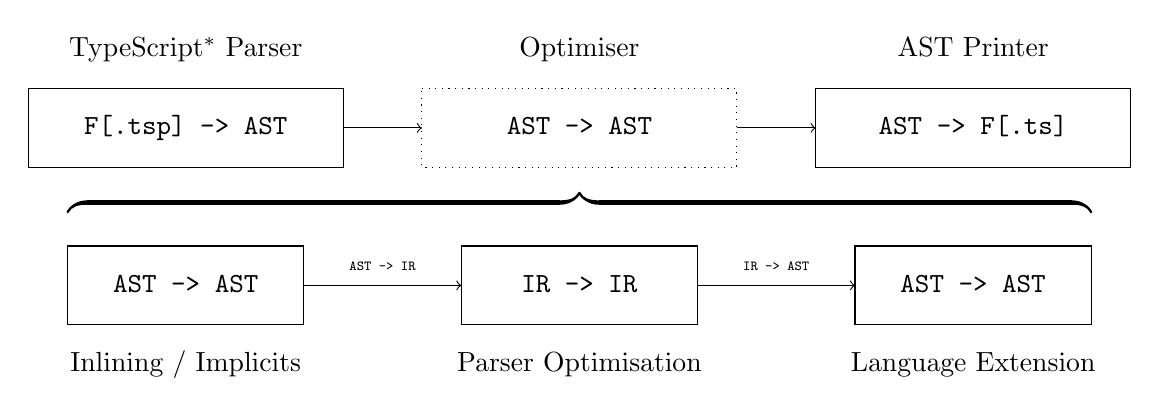
\begin{tikzpicture}[every node/.style={execute at end node=\vphantom{bg}}]
        \begin{scope}[shift={(0, 0)}]
            \node at (0, 0) {\texttt{F[.tsp] -> AST}};
            \node at (0, 1) {\tsext Parser};
            \draw (-2, 0.5) -- (2, 0.5) -- (2, -0.5) -- (-2, -0.5) -- cycle;
        \end{scope}
        \begin{scope}[shift={(5, 0)}]
            \node at (0, 0) {\texttt{AST -> AST}};
            \node at (0, 1) {Optimiser};
            \draw[dotted] (-2, 0.5) -- (2, 0.5) -- (2, -0.5) -- (-2, -0.5) -- cycle;
        \end{scope}
        \begin{scope}[shift={(10, 0)}]
            \node at (0, 0) {\texttt{AST -> F[.ts]}};
            \node at (0, 1) {AST Printer};
            \draw (-2, 0.5) -- (2, 0.5) -- (2, -0.5) -- (-2, -0.5) -- cycle;
        \end{scope}
        \begin{scope}[shift={(0, -2)}]
            \node at (0, 0) {\texttt{AST -> AST}};
            \node at (0, -1) {Inlining / Implicits};
            \draw (-1.5, 0.5) -- (1.5, 0.5) -- (1.5, -0.5) -- (-1.5, -0.5) -- cycle;
        \end{scope}
        \begin{scope}[shift={(5, -2)}]
            \node at (0, 0) {\texttt{IR -> IR}};
            \node at (0, -1) {Parser Optimisation};
            \draw (-1.5, 0.5) -- (1.5, 0.5) -- (1.5, -0.5) -- (-1.5, -0.5) -- cycle;
        \end{scope}
        \begin{scope}[shift={(10, -2)}]
            \node at (0, 0) {\texttt{AST -> AST}};
            \node at (0, -1) {Language Extension};
            \draw (-1.5, 0.5) -- (1.5, 0.5) -- (1.5, -0.5) -- (-1.5, -0.5) -- cycle;
        \end{scope}
        \draw
        (2, 0) edge[->] (3, 0)
        (7, 0) edge[->] (8, 0)
        (1.5, -2) edge[->, above] node{\tiny \texttt{AST -> IR}} (3.5, -2)
        (6.5, -2) edge[->, above] node{\tiny \texttt{IR -> AST}} (8.5, -2);

        \draw[ultra thick, decorate, decoration={calligraphic brace, amplitude=7pt, raise=-2pt}] (-1.5, -1) -- (11.5, -1);
    \end{tikzpicture}
    \vspace{-0.5\baselineskip}
    \caption{Simplified view of the main stages within the preprocessor pipeline, \texttt{F[.x]} denotes a file with extension \texttt{.x}}
    \label{fig:pipeline_diagram}
\end{figure}

The primary entry point for the preprocessor uses \textit{scopt} \cite{scopt} to parse command-line options (see \autoref{tab:cli_opt}), which allows for certain optimisation stages to be enabled / disabled.
Once a file is read in, with the path specified by an argument, the raw input is then parsed by a \tsext parser.
Note that \tsext refers to TypeScript with the additional language features augmented onto the existing grammar (listed in \autoref{sec:lang_ext}).

Once the input file has been successfully parsed, the AST is fed through the optimisation pipeline, detailed further in \autoref{chap:oaa}.
Each `stage', excluding language extensions and IR conversions, is either enabled or disabled, depending on the corresponding configuration option.
Every pipeline stage extends the \texttt{PipelineStage} trait, which provides default AST traversal properties, allowing for a stage to only implement the desired functionality on a subset of the AST, but maintaining the guarantee that everything will be traversed.
The latter is important to ensure that certain assumptions can be made about the AST being fed into subsequent stages.
For example, it is generally safe to assume that any \texttt{Expression}s after the first conversion stage will be \texttt{IR} nodes (detailed in \autoref{sec:ir}).
On overriding a \texttt{PipelineStage}, care should be taken to maintain the behaviour from the superclass (unless explicitly not required) in order to main the traversal properties.

Each of the pipeline stages can access a shared mutable state.
However, pipeline execution typically implies an order of execution: stages cannot simply jump forward in the pipeline and back despite this functionality possibly being beneficial.
For example, the preprocessor may need to report an error to the user and include TypeScript code.
However, without the ability to use later pipeline stages (namely a conversion from the IR to the AST), the functionality for generating code will have to be duplicated.
In order to prevent this, the mutable state can be `locked', thus preventing any changes.

The final stage of the pipeline converts the AST back into a raw string by printing out the AST recursively.
Note that this maintains no formatting, such as indent levels - however, the syntax is now fully valid TypeScript.
Optionally, this raw file can then be passed through a formatter, such as \textit{Prettier} \cite{prettier}.

\section{\texorpdfstring{\tsext}{TypeScript<STAR>} Parser}
\label{sec:ts_parser}
The first stage of the processing pipeline involves parsing the raw input file, which contains a valid (both syntactic and semantic) \tsext program.
Note that the remainder of the pipeline assumes semantic correctness, especially with types, as full type verification lies outside the scope of the preprocessor.

The parser within the preprocessor targets ECMAScript 2015 \cite{es2015spec}, augmented with TypeScript-specific additions from early 2016 \cite{tsls}.
Certain existing language features have been excluded, such as (but not limited to) decorators and ambient declarations.
\textit{Parsley} \cite{willis18} for Scala is used for parsing the raw input into an abstract syntax tree (AST).
The use of a parser combinator library not only seemed natural due to the nature of this library and preprocessor, but also provided numerous benefits, such as the single-pass nature of the lexing, parsing, and construction stages.
One disadvantage of using parser combinators is the lack of error recovery - however, as the preprocessor typically expects correct, well-formed code, this is not a major concern.

Note that the AST contains additional language features not present in TypeScript.
These additions are transformed in subsequent pipeline stages into other AST nodes, which represent valid TypeScript syntax.
In order to recover a valid TypeScript program at the end of the pipeline, each AST node requires a \texttt{print} function, which recursively converts the tree back into program code.
At the end of the pipeline, this is called on a \texttt{Module} representing the entire program, which is then optionally passed into a code formatter.

The entirety of the preprocessing pipeline, bar the formatter which exists externally, is implemented in Scala, in order to leverage its pattern matching abilities, as well as the portability of the JVM (Java Virtual Machine).
The former allows for significantly simpler analysis over the AST, which is hugely beneficial for optimisations on a tree.

\section{Intermediate Representation}
\label{sec:ir}

In lieu of duplicating significant fragments of code to create an entirely separate intermediate representation (IR) to represent the AST, the IR instead extends the existing \texttt{Expression}s, by generating a mapping between the IR and the original or generated \texttt{Expression}.
The inheritance structure of the IR can be seen in \autoref{fig:ir_inheritance} - note that \texttt{Id} also extends \texttt{BindingPattern} and \texttt{PropertyDefinition} from the original TypeScript AST.
By augmenting the existing AST, a separate representation for other parts of the AST, such as statements or declarations, is not required.

\begin{figure}[H]
    \centering
    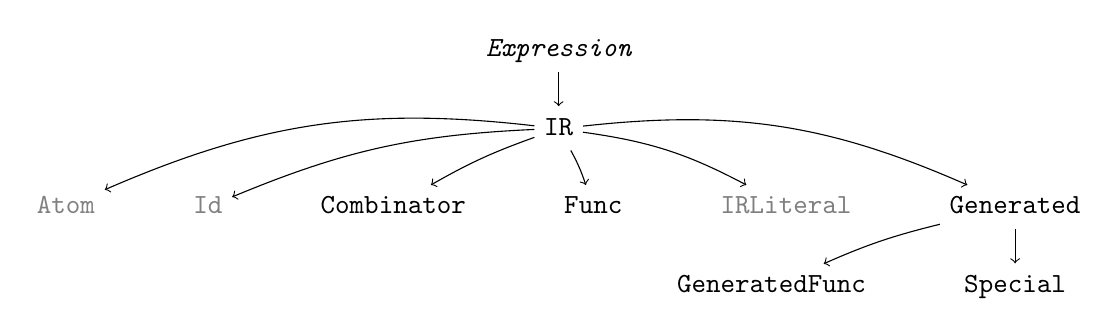
\begin{tikzpicture}[every node/.style={execute at end node=\vphantom{bg}}]
        \node[black!50] at (0, 0) (atom) {\texttt{Atom}};
        \node[black!50, right=of atom] (id) {\texttt{Id}};
        \node[right=of id] (comb) {\texttt{Combinator}};
        \node[right=of comb] (func) {\texttt{Func}};
        \node[black!50, right=of func] (irli) {\texttt{IRLiteral}};
        \node[right=of irli] (gene) {\texttt{Generated}};
        \node (p0) at ($(atom.west)!0.5!(gene.east)$) {};
        \node[] (spec) at (gene |- 0, -1) {\texttt{Special}};
        \node[left=of spec] (gf) {\texttt{GeneratedFunc}};
        \node[] (ir) at (p0 |- 0, 1) {\texttt{IR}};
        \node[] (expr) at (p0 |- 0, 2) {\itshape \texttt{Expression}};
        \draw
        (expr) edge[->] (ir)
        (ir) edge[->, bend right=15] (atom)
        (ir) edge[->, bend right=10] (id)
        (ir) edge[->, bend right=5] (comb)
        (ir) edge[->, bend left=5] (func)
        (ir) edge[->, bend left=10] (irli)
        (ir) edge[->, bend left=15] (gene)
        (gene) edge[->] (spec)
        (gene) edge[->, bend right=5] (gf);
    \end{tikzpicture}
    \caption{Inheritance hierarchy within the IR, nodes in \textcolor{black!50}{\texttt{grey}} are concrete whereas nodes in \texttt{black} are traits}
    \label{fig:ir_inheritance}
\end{figure}

\texttt{Atom}s contain a unique numeric identifier which provides a mapping from an \texttt{Atom} to an \texttt{Expression}, which is stored in a mutable state (implicitly used by all pipeline stages).
These contain any \texttt{Expression}s that cannot be changed into any other representation.
Generally, they contain nodes that require no further inspection, as they are unlikely to contain any combinators - especially not ones that can be meaningfully inspected.

On the other hand, \texttt{Combinator}s are a special case of regular binary operators which contain combinators (any other operation will be converted into an \texttt{Atom}).
For each different combinator, there is a different concrete implementation (\texttt{case class}), allowing for easier inspection in subsequent pipeline stages (via matching on a specific combinator, rather than checking which operation is being performed manually).
Each of these combinators has two arguments, both of which are also IRs.
Similarly, \texttt{Func}s have concrete implementations for reserved functions that are provided with the TypeScript library; these have specific arguments which are assumed to be valid when processing.
This adds the ability to perform some inspection on functions which have known behaviours.

\texttt{Id} and \texttt{IRLiteral} both have similar functionality in that they wrap existing nodes (namely, \texttt{Identifier} and \texttt{Literal}) to work within the IR.
The former is handled separately as it can often be useful to be able to directly access variable names in later stages without the need to reference the shared state (if they were instead represented as \texttt{Atom}s).
On the other hand, \texttt{IRLiteral}s are used for a similar reason, however the main purpose is to allow for inspection into string or character literals, which is useful for subsequent stages.

Finally, the \texttt{Generated} trait refers to any nodes without a mapping from an \texttt{Expression}, meaning that they are only generated by the processing pipeline.
This is further divided into one of two traits.
Nodes which extend the \texttt{GeneratedFunc} trait represent functions that are applied to IR nodes.
These functions have a `fallback' implementation within the library; however, the preprocessor will attempt to directly alter the AST whenever possible.
In contrast, nodes which extend the \texttt{Special} trait are typically used to represent specific values or are used to directly pass information to other stages.
For example, it may be required to explicitly pass an \texttt{Expression} forward without any modifications or highlight characters which exist in the first set of a parser.
\bigskip

The example of addition from \autoref{lst:running_example}, after being parsed into the AST shown in \autoref{lst:running_ast}, is translated into the IR as shown in \autoref{lst:running_ir}.
Notice how only the information that is directly related to parsers is maintained, whereas the function is simply converted into \texttt{Atom(0)}.

\begin{capminted}
    \begin{minted}{scala}
        (Id("expr") <**> (Atom(0) <$ Chr(IRLiteral("'+'"))) <*> Id("nat")) <|>
        Id("nat")
    \end{minted}
    \vspace{-0.5\baselineskip}
    \caption{IR of right-hand side of assignment}
    \label{lst:running_ir}
\end{capminted}

\subsection{Function Rewriting}
\label{ssec:func_rewrite}
An example of the function rewriting is as follows, where \texttt{f0} is a function without AST rewriting (uses library functions) and \texttt{f1} is a function that is directly rewritten.
While this may seem like a pathological example, these transformations are used extensively when rewriting the parsers to support left-recursion.

\begin{capminted}
    \begin{minted}{typescript}
        let f0 = flip(curry(unpairFirstArg(
            ([x, y]: [number, number], z: number) => x + y - z
        )));
        let f1 = ([y, z]: [number, number]) => (x: number) => x + y - z;
    \end{minted}
    \vspace{-0.5\baselineskip}
    \caption{Example of function rewriting performed by the preprocessor}
    \label{lst:rewrite_xyz}
\end{capminted}

Not only does the direct rewrite improve code clarity by omitting multiple function calls, there is also a small but measurable performance uplift stemming from the reduced number of invocations.
This can be seen in \autoref{fig:rewrite}, which performs $10,000$ iterations of the function in \autoref{lst:rewrite_xyz}.
Within each iteration, the function is transformed and executed $n$ times.
This result demonstrates that with repeated invocations, the performance gap between the two forms becomes narrower.
However, the directly rewritten form consistently performs better, especially with few invocations when it can complete execution in approximately half the time.

\begin{figure}[H]
    \centering
    \import{figs}{figs/gen_func_rewrite.pgf}
    \vspace{-0.5\baselineskip}
    \caption{Change in average execution time based on number of repetitions}
    \label{fig:rewrite}
\end{figure}

\section{Language Extensions}
\label{sec:lang_ext}

\def\mplw{0.49\textwidth}
\def\mprw{0.49\textwidth}

As part of the preprocessor, a number of languages features are implemented that augment the existing TypeScript grammar, most of which are implemented to provide `syntactic sugar' for writing parser combinators.
This section introduces these additions alongside some context surrounding usage.
Note that for all the subsequent code snippets in this section, the snippet on the left refers to the augmented grammar (\texttt{.tsp}) and the snippet on the right refers to the transpiled TypeScript (\texttt{.ts}).

\subsection{Declarations}
Two new lexical declarations have been added, namely \texttt{val} and \texttt{lazy}.
The former is simply an alias for \texttt{const}, with no additional functionality.
On the other hand, \texttt{lazy} allows for rudimentary laziness, thus allowing for parsers to be recursively defined - required for supporting recursive syntax.
This can be seen in the example below, where \texttt{p} references itself.
Without the additional wrapping for laziness, the code would be semantically invalid as a variable would be used prior to its assignment.

\begin{center}
    \begin{minipage}[t]{\mplw}
        \begin{minted}{teaspoon_lex.py:TeaspoonLexer -x}
            lazy p = p;
            val q = x;
        \end{minted}
    \end{minipage}
    \hfill
    \tikzmark{lt_d}
    \hfill
    \begin{minipage}[t]{\mprw}
        \begin{minted}{typescript}
            const p = lazy(() => p);
            const q = x;
        \end{minted}
    \end{minipage}
\end{center}
\tikz[remember picture] \node[overlay] at ($(pic cs:lt_d) + (-0.5, -0.25)$) {$\leadsto$};

\subsection{User-Defined Operators}
In order to provide an intuitively legible syntax for writing parsers, user-defined operators have been implemented.
Note that the snippet below does not provide usage for all implemented operators, but rather demonstrates how they are supported.
In the example, \texttt{p} is an example of how a simple combinator is written into a function call.
The left-associative property of combinators is also respected, as shown in \texttt{q}, with support for parentheses shown in \texttt{s}.
Similarly, the lower precedence of the choice combinator (\texttt{\choice}) is shown in \texttt{r}.
Finally, arbitrary user-defined functions can be supported, as shown in \texttt{t} - this addition allows for combinators to be defined beyond what is provided by the library, without requiring changes to the preprocessor.

\begin{center}
    \begin{minipage}[t]{\mplw}
        \begin{minted}{teaspoon_lex.py:TeaspoonLexer -x}
            let p = a <~> b;
            let q = a *> b *> c;
            let r =
              a <*> b <|> c <*> d;
            let s =
              a <**> (pf <* b) <*> c;
            let t = a <xyz> b;
        \end{minted}
    \end{minipage}
    \hfill
    \tikzmark{lt_udo}
    \hfill
    \begin{minipage}[t]{\mprw}
        \begin{minted}{typescript}
            let p = mult(q, r);
            let q = apR(apR(a, b), c);
            let r =
              choice(ap(a, b), ap(c, d));
            let s =
              ap(pa(a, apL(pf, b)), c);
            let t = xyz(a, b);
        \end{minted}
    \end{minipage}
\end{center}
\tikz[remember picture] \node[overlay] at ($(pic cs:lt_udo) + (-0.5, -1.375)$) {$\leadsto$};

\subsection{Implicit Conversions}
In order to reduce the amount of conversion the user has to manually perform, implicit conversions can be enabled in the pipeline.
With this enabled, a use of a string, character, or regular expression literal in place of where a parser is expected will cause the preprocessor to automatically apply a conversion (wrapping the function with \texttt{chr}, \texttt{str}, or \texttt{re}, depending on the type of the literal).
This addition provides some ability to have `overloaded strings', as described by Willis \& Wu (2021) \cite{willis21}.

\begin{center}
    \begin{minipage}[t]{\mplw}
        \begin{minted}{teaspoon_lex.py:TeaspoonLexer -x}
            let p = f <*> 'a' <*> /b/i;
            let q = 'c' $> 'd';
            let r = attempt('ef');
        \end{minted}
    \end{minipage}
    \hfill
    \tikzmark{lt_ic}
    \hfill
    \begin{minipage}[t]{\mprw}
        \begin{minted}{typescript}
        let p =
          p(ap(f, chr('a')), re(/b/i));
        let q =
          constFmapR(chr('c'), 'd');
        let r = attempt(str('ef'));
        \end{minted}
    \end{minipage}
\end{center}
\tikz[remember picture] \node[overlay] at ($(pic cs:lt_ic) + (-0.5, -0.85)$) {$\leadsto$};

\subsection{`Macros'}
\label{ssec:inline}
One limitation of the preprocessor, when performing analysis, is observing the behaviour of more `complex' functions or declarations.
While it may be feasible to inline some variable declarations, if they are known to be immutable, it can often negatively impact the readability of the produced code.
It may not be desirable to inline a complex declaration.
On the other hand, it is likely difficult to analyse an arbitrary function, even if the underlying semantics are fairly simple.
For example, consider the function \texttt{between}, provided in the library.
The invocation \texttt{between(l, p, r)} simply denotes \texttt{l \apr p \apl r} - in this case, the function is simply shorthand.
For these cases, the user should be able to specify when a replacement can be safely performed, via the use of the \texttt{inline} `declaration'.

\begin{center}
    \begin{minipage}[t]{\mplw}
        \begin{minted}{teaspoon_lex.py:TeaspoonLexer -x}
            inline paap(x, y, z) =
              x <**> y <*> z;
            inline o = add <$ chr('+');
            inline add = (x: number) =>
              (y: number) => x + y;

            let r = paap(a, o, b);
        \end{minted}
    \end{minipage}
    \hfill
    \tikzmark{lt_m}
    \hfill
    \begin{minipage}[t]{\mprw}
        \begin{minted}{typescript}
            let r = ap(pa(a,
              constFmapL(
                (x: number) =>
                  (y: number) => x + y,
                chr('+'))
            ), b);
        \end{minted}
    \end{minipage}
\end{center}
\tikz[remember picture] \node[overlay] at ($(pic cs:lt_m) + (-0.5, -1.375)$) {$\leadsto$};

The snippet demonstrates how a substitution is performed, for substitutions with and without parameters.
Notice that the substitution is not restricted to only parsers, as seen with \texttt{add}.
It is important to note that this does not perform a na\"ive text replacement, but rather recursively splices in parts of the AST.
By modifying the AST, further analysis can be performed in subsequent stages.
For example, rather than seeing \texttt{r} as being an arbitrary function call, which may have behaviour that cannot trivially be inspected, it is seen as a combinator tree which can be analysed further.
The ability to provide these `hints' to the preprocessor is beneficial to the efficacy of optimisations that analyse combinator trees.

Consider the earlier example of \texttt{between}.
Note that \texttt{p = between(l, a, r)} and \texttt{q = between(l, b, r)} follow a similar form.
However, without knowing how \texttt{between} is defined, it is not trivial to deduce that both \texttt{p} and \texttt{q} share a common prefix.
On the other hand, if both were expanded based on the inline definition, it is trivial to see that both parsers have a common prefix and suffix of \texttt{l} and \texttt{r}, respectively.


\section*{Summary}
This chapter demonstrates how the raw \tsext source code is transformed in order to support numerous language features, including the user-defined operators introduced in \autoref{chap:library}.
The additions to TypeScript are also presented in the context of parser combinators and how a user may find them beneficial.
A deeper dive was also made into the underlying design of the preprocessor itself as well as how the parsed structure is traversed and simplified for optimisations.

However, the theory and implementation of the optimisation steps have been omitted for brevity.
Instead, they are further explored in \autoref{chap:oaa}, which dives deeper into the techniques applied and how they transform the grammar.

\chapter{Optimisation and Analysis}
\label{chap:oaa}

The optimisation stage, introduced in \autoref{chap:preprocessor}, forms the crux of the preprocessor.
This chapter provides a deeper insight into each of the various optimisations and how they can remedy common pitfalls present in parser combinators.
These optimisations include simple changes to the parsers via parser laws to simplify the combinator tree, as well as deeper optimisations which can alter the semantics such as rewriting a grammar to support left recursion.
Multiple optimisations that aid in improving performance from backtracking are also explored, including a specific case for alternative strings as well as a more generalised case on combinators.

\section{Simple Optimisations}
\label{sec:simple_opt}

\subsection{Choice Reduction}
\label{ssec:choice_reduce}

A common pattern in parsers and grammars are sequences of alternatives, or disjunctions.
Since choice (\texttt{\choice}) is an associative operator, it can often be useful to treat a tree of alternatives as a sequence, which can be reconstructed in a fully left-associative manner.
Note that the order should generally be maintained, as it is not a commutative operator.

While this property is primarily used in subsequent optimisations, it can enable a simple optimisation - removing duplicate disjunctions.
For example, if a parser was \texttt{p \choice q \choice p}, it could be simply reduced to \texttt{p \choice q}.
However, by trimming down disjunctions, it reduces the amount of processing required in subsequent steps, most of which rely on dealing with sequences of disjunctions.

\subsection{Parser Law Optimisation}
\label{ssec:parser_law}

In order to simplify the parsers further, before more complex optimisations are applied, basic destructive transformations can be performed.
Note that this step does not apply all optimisation rules, even if it may allow for further optimisation - it only makes changes that will reduce the size of the parser.
Consider the size of the parser as the number of nodes in the combinator tree.
Generally, this refers to the neutral, catch, and absorption laws of alternatives, applicatives, and monoidals (previously discussed in \autoref{ssec:alternative}).
However, this step also applies the definition of `fmap' when applicable - by performing this reduction, it allows for subsequent preprocessing stages to easily determine whether something is a parser or not.

\section{Left Recursion Analysis}
\label{sec:lrec_analysis}

A common pitfall of recursive descent parsers, and by extension parser combinators, is the inability to handle left-recursion.
While techniques exist to manually manipulate a grammar, they can often be mechanical and slow.
Additionally, parser combinators typically contain significantly more information than just the parsing structure, often including semantics on how subtrees (of parsers) should be combined.
This section introduces how left recursion can automatically be detected and rewritten in a form that can terminate via iteration \cite{willis21}, while preserving the desired, user-defined semantics.

\subsection{First Sets}
\label{ssec:first_sets}

In order to begin analysing left recursion, the first step is to determine a programmatic method of checking if a production is left-recursive in the first place.
More importantly, the alternatives (if any) that are not left-recursive also need to be deduced.

The first set of a production can be intuitively thought of as anything that can begin the derivation for a particular rule.
In a traditional grammar, this is simply a union over the first sets of all disjunctions (alternatives) of a rule.
The first set of a rule without disjunctions is the first set of the first element in the rule, which can then be recursively computed.
Finally, the first set of a terminal is a set containing only itself.
The same intuition can be carried forwards to parser combinators.

Let $\mathcal{F}$ represent the \textbf{global} first set and $\mathcal{L}$ represent the \textbf{local} first set.
The local first set is defined as follows on combinators (note that $\texttt{i}_\texttt{0}$ denotes the first character of the string literal that \texttt{i} represents (which can be an escape sequence) and \texttt{<X>} denotes any arbitrary combinator):
\begin{align*}
    \mathcal{L}(\texttt{p \choice q}) & = \mathcal{L}(\texttt{p}) \cup \mathcal{L}(\texttt{q}) & \text{union for choice} \\
    \mathcal{L}(\texttt{f \constfmapl p})\ |\ \mathcal{L}(\texttt{f \fmap p}) & = \mathcal{L}(\texttt{p}) & \text{non-parser on left} \\
    \mathcal{L}(\texttt{p \constfmapr f})\ |\ \mathcal{L}(\texttt{p \pamf f}) & = \mathcal{L}(\texttt{p}) & \text{non-parser on right} \\
    \mathcal{L}(\texttt{pure x <X> p}) & = \mathcal{L}(\texttt{p}) & \text{\texttt{pure} ($\varepsilon$) first} \\
    \mathcal{L}(\texttt{p <X> q}) & = \begin{cases}
        \mathcal{L}(p) & \text{if } \mathcal{L}(p) \neq \varnothing \\
        \mathcal{L}(q) & \text{otherwise}
    \end{cases} & \text{any other combinator} \\
    \mathcal{L}(\texttt{pure x})\ |\ \mathcal{L}(\texttt{empty}) & = \varnothing & \text{empty set} \\
    \mathcal{L}(\texttt{i: Id}) & = \{ \texttt{i} \} & \text{`terminal'}\\
    \mathcal{L}(\texttt{a: Atom}) & = \{ \texttt{a} \} & \text{`terminal'} \\
    \mathcal{L}(\texttt{i: IRLiteral}) & = \begin{cases}
        \{ \texttt{i}_\texttt{0}, \texttt{i} \} & \text{if string / char} \\
        \{ \texttt{i} \} & \text{otherwise}
    \end{cases} & \text{`terminal'}
\end{align*}

The computation of the local first set is done via the use of pattern matching in Scala, with recursion when required.
Also note that the results of the first set computation is memoised in the shared mutable state, preventing a possibly expensive recomputation at the cost of space.

Note that the computation for the first set of a function is similar, by looking at the first parser in the function's arguments.
One important distinction is that the local first set considers identifiers, which are typically references to other parsers (productions), as a terminal, which is incorrect.
While this alone allows for some simple left-recursive productions to be detected, it does not yet fully account for indirect left recursion.
As the preprocessor has a wider view of the program, it is feasible to obtain the global first set of all productions.

Consider all lexical declarations that can occur in the program.
Looking at only parsers (other declarations will have a first set computed, but are meaningless), a declaration refers to any statement that declares a value (reassignments are not supported), such as \texttt{p = q}.
In this case, \texttt{p} is the parser of interest, which is an identifier assignment.
The value of the assignment, \texttt{q}, can be in any of the forms listed above, including disjunctions.

A relation $L$, where $\langle p, a \rangle$ denotes $a$ (a parser) as being in the \textbf{local} first set of $p$ (an identifier), is defined as the following:

$$L = \{ \langle p, a \rangle\ |\ a \in \mathcal{L}(p) \}$$

The global first set can then be computed as the \emph{transitive closure} of $L$, such that $\mathcal{F} = L^+$.
Note that the transitive closure $L^+$ refers to the smallest transitive set containing $L$.
A binary relation $R$ on \texttt{IR} is defined as transitive if for all $p, q, r \in \texttt{IR}$ if $\langle p, q \rangle$ and $\langle q, r \rangle$ both exist, then $\langle p, r \rangle$ must exist, or formally:

$$\forall p, q, r \in \texttt{IR}\ [\langle p, q \rangle \in R \land \langle q, r \rangle \in R \Rightarrow \langle p, r \rangle \in R]$$

This can be computed by adding `missing' tuples by repeatedly performing relation composition until the relation is transitive.
As each step of adding missing tuples is required for transitivity, this creates the minimal set - the transitive closure.
In practice, this computation is done by first scanning the entire program's AST for declarations and computing the local first set, creating a mapping from \texttt{String} (the identifier) to \texttt{Set[IR]}.
The transitive closure is then computed by iteratively expanding any identifiers found in a first set to the identifier's respective first set until all identifiers (in the expanded first set) have been visited.

Consider the following example of a parser that contains indirect left recursion:

\begin{minted}{teaspoon_lex.py:TeaspoonLexer -x}
    val a  = '1' $> 1;
    lazy p = f <$> q <*> a <|> a;
    lazy q = p <* '+';
\end{minted}

The following result is obtained, using the rules for \textbf{local} first sets and the subsequent construction of $\mathcal{F}$.
Note that expansion is an iterative process, as seen in $\mathcal{F}(\texttt{q})$, where the expansion of \texttt{p} leads to further expansion on \texttt{a}.
\begin{align*}
    \mathcal{L}(\texttt{a}) & = \{ \texttt{'1'} \} \\
    \mathcal{L}(\texttt{p}) & = \{ \texttt{q}, \texttt{a} \} \\
    \mathcal{L}(\texttt{q}) & = \{ \texttt{p} \} \\
    \mathcal{F}(\texttt{a}) & = \{ \texttt{'1'} \} & \text{no identifiers} \\
    \mathcal{F}(\texttt{p}) & = \{ \texttt{p}, \texttt{q}, \texttt{a}, \texttt{'1'} \} & \texttt{q} \mapsto \{ \texttt{q}, \texttt{p} \}, \texttt{a} \mapsto \{ \texttt{a}, \texttt{'1'} \} \\
    \mathcal{F}(\texttt{q}) & = \{ \texttt{p}, \texttt{q}, \texttt{a}, \texttt{'1'} \} & \texttt{p} \mapsto \{ \texttt{p}, \texttt{q}, \texttt{a} \} \mapsto \{ \texttt{p}, \texttt{q}, \texttt{a}, \texttt{'1'} \}
\end{align*}

\subsection{Detection}
\label{ssec:lrec_detection}

By computing the first sets $\mathcal{F}$, it is now possible to detect all three forms of left recursion; direct (from the local first set), indirect (via the transitive closure on local first sets), and hidden (via the rules in place to deal with $\varepsilon$).
Recall that a parser is left-recursive when it is able to derive some form, after some number of substitutions (or none), with itself as the first parser \cite{power99}.
Intuitively, this means left recursion occurs when a parser contains a rule where the derivation begins with itself.
As such, a parser \texttt{p} is left-recursive if it is contained within its own first set; $\texttt{p} \in \mathcal{F}(\texttt{p})$.

However, simply detecting a parser is left-recursive is not enough to begin rewriting it.
The more common form is as follows, where some rules ($\texttt{r}_\texttt{i}$) are left-recursive, but others ($\texttt{q}_\texttt{j}$) are not:

\begin{capminted}
    \begin{minted}{teaspoon_lex.py:TeaspoonLexer -x}
        lazy p = r_1 <|> ... <|> r_m <|> q_1 <|> ... <|> q_n;
    \end{minted}
    \vspace{-0.5\baselineskip}
    \caption{Example of parser \texttt{p} in a general form}
    \label{lst:p_general}
\end{capminted}

In order to rewrite the structure of \texttt{p}, the disjunctions must first be partitioned into those which are locally left-recursive (\texttt{R}) and those which are not (\texttt{Q}).
Note that the use of $\text{disjunctions}(\texttt{p})$ refers to the set of alternatives for \texttt{p}.
\begin{align*}
    \text{disjunctions}(\texttt{p}) & = \{ \texttt{r}_\texttt{1}, \dots, \texttt{r}_\texttt{m}, \texttt{q}_\texttt{1}, \dots, \texttt{q}_\texttt{n} \} & \text{from example above} \\
    \texttt{R} & = \{ \pi \in \text{disjunctions}(\texttt{p})\ |\ p \in \mathcal{L}(\pi) \} \\
    \texttt{Q} & = \{ \pi \in \text{disjunctions}(\texttt{p})\ |\ p \notin \mathcal{L}(\pi) \}
\end{align*}

The use of local left recursion (rather than global) allows for safer restructuring - hoisting in declarations may lead to unintended consequences as well as generally more verbose, thus less legible, generated code.
In order to allow for declarations that can be safely hoisted in, the lexical declaration \texttt{inline} has been implemented, as mentioned in \autoref{ssec:inline}.
As such, all three forms of left recursion can be detected, however, only direct left recursion can be rewritten.
The other forms are quite infrequent in most grammars, as mentioned in Parr et al. (2014) \cite{parr14}.

\subsection{Rewriting}
\label{ssec:lrec_rewrite}
It is important to note that by rewriting the productions, the preprocessor will fundamentally alter the semantics of these parsers.
Parsers which previously would not terminate due to infinite recursion are now modified to parse iteratively, with termination being possible.

This is done in three steps; normalisation, reduction, and finally, rewriting.
The underlying idea behind rewriting left recursion is to convert a `standard' production into a parser that utilises \texttt{postfix}.
Note that \texttt{postfix} was chosen (rather than \texttt{infixl}, or similar \cite{willis21}) as it provided the most `general' form - it is able to automatically handle infix operators as well as postfix operators.
This property is desirable, especially in the context of automatic rewriting; while the generated program may be less concise, it allows for more forms of detection, as well as a reduced likelihood of errors, thus requiring less manual intervention.

Consider the following (direct) left-recursive production, similar to the previous declaration of \texttt{p};
$$P \to \underbrace{\overbrace{Ps_1}^{r_1}\ |\ \dots\ |\ \overbrace{Ps_m}^{r_m}}_{\texttt{R}}\ |\ \underbrace{q_1\ |\ \dots\ |\ q_n}_{\texttt{Q}}$$

On a translation to a PEG, the recursive productions simply become repetition operators as stated in Ford (2004) \cite{ford04}, thus the following result is obtained (CFG to PEG);
$$P \leftarrow (q_1\ /\ \dots\ /\ q_n)(s_1\ /\ \dots\ /\ s_m)*$$

This result is similar to that of Hill (1994) \cite{hill94}.
Note that $P$ may appear in $s_j$, such as in the case of addition ($E \to E \texttt{ '+' } E$) where $P = E$ and $s_j = \texttt{'+' } E$.
However, the rewriting remains valid as long as $P \notin \mathcal{F}(s_j)$.
Note that the rewrite still occurs if $P \in \mathcal{F}(s_j)$ but $P \notin \mathcal{L}(s_j)$, however, the preprocessor will raise a warning regarding a possible indirect or hidden left recursion.

However, this translation of a CFG to a PEG must be mirrored in terms of parser combinators, which not only carries syntactic information in terms of the parse structure, but has underlying semantics in terms of how the parsed results are used (or not used).
This raises a number of challenges: the same grammar can exist in multiple forms (lack of normalisation) and combinators carry semantic information as well as syntactic information.

The first of which is that parser combinators can exist in a number of forms which represent the same underlying grammar.
For example, the four following combinators all represent $P_i \to P_i S\ |\ Q$:

\begin{minted}{teaspoon_lex.py:TeaspoonLexer -x}
    lazy p_0 = f_0 <$> p_0 <*> s <|> q;
    lazy p_1 = p_1 <**> pure(f_1) <*> s <|> q;
    lazy p_2 = f_2 <$> p_2 <~> s <|> q;
    lazy p_3 = lift2(f_3, p_3, s) <|> q;
\end{minted}

The second problem is preserving the semantics of the parse - note that in the example above, there is an additional transformation that is applied to each of the $P_i S$ disjunctions.
While it may be quite intuitive to reason about the behaviour of the function at a glance, any changes to the parser, which may be numerous, must be accurately reflected in how the function is transformed (recall the rewriting of certain functions from \autoref{ssec:func_rewrite}).
Without this constraint, a rewritten parser would simply verify if the structure is correct and give the sequence of parsers applied - this is only sufficient for recognisers.
While parser generators will still require tree reassociation, the semantics are provided `externally' (outside the parser generator) over the parse tree, which is not the case for parser combinators.

\subsubsection*{Normalisation}
The first problem is addressed via normalisation and reduction.
In order to aid the subsequent steps, any locally left-recursive parsers are matched against a series of patterns in order to extract the required elements.
The chosen normal form for the majority of operators is $\texttt{p} = \texttt{lift2(f, q, r)}$ - this allows for a clear separation between three key components; \texttt{f} (an uncurried function), \texttt{q} (the left recursion), and \texttt{r} (the `remainder' or suffix).
Notice that the left recursion does not necessarily have to be \texttt{p} - just that $\texttt{p} \in \mathcal{L}(\texttt{q})$.

Note that any patterns using `reverse fmap' (\texttt{\pamf}) will be omitted for brevity; simply replace a use of \texttt{f \fmap p} with \texttt{p \pamf f}, additionally patterns using `const fmap' such as \texttt{x \constfmapl p} can be substituted with \texttt{p \constfmapr x}.
Some normalisation patterns are as follows:

\begin{capminted}
    \begin{minted}{scala}
        p match {
            case (f <$> q) <*> r          => Lift2(Uncurry(f), q, r)
            case (f <$> (q <~> r))        => Lift2(ArgsToTuple(f), q, r)
            case (q <**> Pure(f)) <*> r   => Lift2(Uncurry(f), q, r)
            case q <**> (f <$> r)         => Lift2(Uncurry(Flip(f)), q, r)
            case (q <**> (f <$ op)) <*> r => Lift2(Uncurry(f), q, op *> r)
            // ...
        }
    \end{minted}
    \vspace{-0.5\baselineskip}
    \caption{Examples of normalisation steps for common patterns}
    \label{lst:scala_normalisation}
\end{capminted}

While these patterns cannot account for every possible combination, when coupled with the later reduction steps, they can deal with a variety of parsers in various common forms.
The validity of these normalisation steps is detailed in \autoref{sec:sound_normalisation}.

\subsubsection*{Reduction}
Recall that the recursive component of $\texttt{p} = \texttt{lift2(...)}$ does not necessarily have to be \texttt{p}.
However, the end goal is to `reduce' this component down to just be \texttt{p}.
This is done via a sequence of reduction steps, which monotonically simplifies the recursive component; the complexity of a component can be quantified as the size of the combinator tree representing it.
By requiring a constraint where the structure is monotonically simplified, termination is guaranteed - resulting in a successful reduction or a failed reduction (which causes the preprocessor to roll back any transformations made on a particular disjunction).

Similar to the normalisation step, some patterns will be omitted for brevity if they are equivalent to another pattern, albeit with flipped arguments.
Additionally, \texttt{\apl} and \texttt{\multl} are equivalent and thus have the same reduction rules.
Function shorthand will also contain \texttt{UFA(f)} and \texttt{MFA(f)} to represent \texttt{UnpairFirstArg(f)} and \texttt{MapFirstArg(f)}, respectively.

\begin{capminted}
    \begin{minted}{scala}
        p match {
            case Lift2(f, r <* s, q)   => _Lift2(f, r, s *> q)
            case Lift2(f, g <$> r, q)  => _Lift2(MFA(g, f), r, q)
            case Lift2(f, c <$ r, q)   => _Lift2(MFA(Const(c), f), r, q)
            case Lift2(f, r <~> s, q)  => _Lift2(UFA(f), r, s <~> q)
            case Lift2(f, r <*> s, q)  => _Lift2(f, AFM <$> (r <~> s), q) // (1)
            case Lift2(f, r <**> s, q) => _Lift2(f, PFM <$> (r <~> s), q) // (1)
            case Lift2(f, r <:> s, q)  => _Lift2(f, ((:) <$> r) <*> s, q) // (2)
            // ...
        }
    \end{minted}
    \vspace{-0.5\baselineskip}
    \caption{Some \texttt{lift2} reduction cases, note that \texttt{\_Lift2} is a `smart constructor' that performs further reductions}
    \label{lst:scala_reduction}
\end{capminted}

The validity of these reductions is proven via equivalences in \autoref{sec:sound_reductions}.
Note that the rules for \texttt{\ap} and \texttt{\pa} bootstrap off of the existing reduction steps for \texttt{\mult} and \texttt{\fmap}, based on the idea of recovering applicative from monoidal, as stated by McBride \& Paterson (2008) \cite{mcbride08}.
As such, the reduction is implemented in a way that adds complexity to begin with but reduces in a fixed, finite number of steps to a simpler form, thus maintaining the monotonically decreasing constraint.
The same idea is applied for \texttt{<:>} (lifted cons), however this also builds on the use of \texttt{\ap}.

\subsubsection*{Postfix}

Prior to this point, the parsers were still left-recursive.
Nothing has been done to change the semantics yet, however left-recursive disjunctions have been `reconditioned'; the aforementioned problems (the lack of a normal form and the preservation of parse semantics) have been dealt with.
Recall the earlier example of \texttt{p}, shown in \autoref{lst:p_general}.
In the ideal case, this parser would have become reconditioned to the following;
\begin{capminted}
    \begin{minted}{teaspoon_lex.py:TeaspoonLexer -x}
        lazy p = lift2(f_1, p, s_1) <|> ... <|> lift2(f_m, p, s_m) <|>
                 q_1 <|> ... <|> q_n;
    \end{minted}
    \vspace{-0.5\baselineskip}
    \caption{Example of parser \texttt{p}, after normalisation and reduction}
    \label{lst:p_norm_reduce}
\end{capminted}

Using the previous partitioning of \texttt{Q} and \texttt{R}, where the latter represents left-recursive disjunctions, it follows that the newly created \texttt{lift2}s fall into the \texttt{R} partition.
Note that \texttt{postfix} and \texttt{lift2} have the following types - additionally, in the case of \texttt{lift2} there is the constraint that $\texttt{C} = \texttt{A}$, as \texttt{p} has the type \texttt{P<A>}.

\begin{capminted}
    \begin{minted}{typescript}
        function postfix(q: P<A>, op: P<(a: A) => A>): P<A>;
        function lift2(f: (a: A, b: B) => C, p: P<A>, q: P<B>): P<C>;
    \end{minted}
    \vspace{-0.5\baselineskip}
    \caption{Types involved for postfix conversion}
    \label{lst:conv_types}
\end{capminted}

Using these types as guide, the next natural step is to populate the parameters of \texttt{postfix} as required, resulting in a parser that replaces recursion with iteration.
The semantics of \texttt{postfix} are that it parses one \texttt{q} and then zero or more occurrences of \texttt{op}, applying the result to some accumulating value.
Naturally, \texttt{q} must be the non-recursive cases found in the \texttt{Q} partition.
However, \texttt{Q} represents a collection of parsers, which can trivially be changed into a parser by reducing as alternatives (\texttt{\choice}).

The remaining work lies in converting the recursive cases into \texttt{op}s (which can then be reduced in the same way).
Recall that work was done to ensure that \texttt{lift2} followed the same structure, where \texttt{p} is isolated in all alternatives.
Consider a single recursive disjunction, $\texttt{lift2(f, p, s)} \in \texttt{R}$.
If the value for \texttt{b} (the second argument) were to be pre-populated in \texttt{f}, the resulting function would be ideal for \texttt{postfix}.

This can be seen in \autoref{lst:sub1_p}, where the parser simply subtracts 1 from the number parsed.
In this example, the argument \texttt{b} is represented by \texttt{y}.
However, it is clear that this will be 1: the result of the second `parser' (\texttt{pure(1)}).
If this value were to be populated, the resultant function would resemble \texttt{(x: number) => x - 1}, which is the desired effect.
Of course, this would have to be done to accommodate an arbitrary parsed result, not just a constant.

\begin{capminted}
    \begin{minted}{typescript}
        let sub1 = lift2((x: number, y: number) => x - y, nat, pure(1));
    \end{minted}
    \vspace{-0.5\baselineskip}
    \caption{Simple example of \texttt{lift2} to demonstrate pre-populating an argument}
    \label{lst:sub1_p}
\end{capminted}

This is done by first currying \texttt{f}, which has the type \texttt{(a: A) => (b: B) => A}.
By flipping this curried function, the resultant type is \texttt{(b: B) => (a: A) => A}.
Finally, this can be partially applied with `fmap' (\texttt{\fmap}), with the result (\texttt{flip(curry(f)) \fmap r}) being of the desired type.
This transformation is performed on all alternatives in \texttt{R}, which is then reduced.
Validity of this transformation is further discussed in \autoref{sec:sound_rewrite}.

The earlier example, shown in \autoref{lst:p_general} and \autoref{lst:p_norm_reduce}, is finally rewritten into:
\begin{capminted}
    \begin{minted}{teaspoon_lex.py:TeaspoonLexer -x}
        lazy p = postfix(q_1 <|> ... <|> q_n,
            flip(curry(f_1)) <$> s_1 <|> ... <|>
            flip(curry(f_m)) <$> s_m
        );
    \end{minted}
    \vspace{-0.5\baselineskip}
    \caption{Example of parser \texttt{p}, after rewriting}
    \label{lst:p_rewrite}
    \vspace{-\baselineskip}
\end{capminted}

\subsection{Worked Example}
\label{ssec:worked_ex}

Recall the example of addition first introduced in \autoref{lst:running_example} and the subsequent IR in \autoref{lst:running_ir}.
The code matches the pattern \texttt{q \pa (f \constfmapl op) \ap r} exactly, with no requirement for reduction.
In this case (let \texttt{C('+')} denote \texttt{Chr(IRLiteral("'+'"))} for brevity):

\begin{center}
    \vspace{-2\baselineskip}
    \begin{minipage}[t]{0.49\textwidth}
        \begin{align*}
            \texttt{q} & = \texttt{Id("expr")} \\
            \texttt{f} & = \texttt{Atom(0)}
        \end{align*}
    \end{minipage}
    \hfill
    \begin{minipage}[t]{0.49\textwidth}
        \begin{align*}
            \texttt{op} & = \texttt{C('+')} \\
            \texttt{r} & = \texttt{Id("nat")}
        \end{align*}
    \end{minipage}
\end{center}

Trivially, this is converted into \texttt{lift2(u(f), Id("expr"), C('+') \apr Id("nat"))}.
As this is already in the desired shape, where the left recursion is the first parser, it can be converted into a \texttt{postfix} operation.
This is then rewritten into the following (the \violet{violet} component is the result of the function after converting from the IR):

$$\underbrace{\texttt{flip(curry(u(f)))}}_{\violet{\texttt{(y) => (x) => x + y}}} \texttt{ \fmap (C('+') \apr Id("nat"))}$$

Notice how the first application, which would be to the result of \texttt{Id("nat")}, is the argument \texttt{y}, thus pre-populating the function as desired.
\section{String Trie}
\label{sec:str_trie}

A frequently observed pattern in parsing, especially in programming languages, is a number of alternative strings, namely keywords.
However, this pattern can often lead to two pitfalls; the first revolves around the ordering of words and the second revolves around the performance penalty caused by backtracking.
The execution of disjunctions in parser combinators follows the behaviour of PEGs.
As such, the `dangling else ambiguity' can be easily resolved by a reordering of disjunctions, with the longest pattern first.
This also means that disjunctions are not commutative (therefore, this optimisation changes the semantics of the parser).
Consider an example consisting of a subset of TypeScript keywords:

\begin{lstlisting}
    kw ::= 'as' | 'async' | 'break' | 'case' | 'const' | 'continue'
\end{lstlisting}

In this order, if the word \texttt{'async'} were to be parsed, the parser would terminate on a successful parse of \texttt{'as'}, with a remainder of \texttt{'ync'}.
On the other hand, if the order were to be flipped, with \texttt{'as'} being after \texttt{'async'}, the parser would fail due to the input being partially consumed - backtracking is therefore required to reset the state back to where the first parser began.
However, backtracking operations are inherently expensive, possibly requiring work to be redone.
Ideally, a parser would have minimal (if any) backtracking (implemented via the use of \texttt{attempt}), and any parsers that contain backtracking would be as `small' as possible.

As noted in Swierstra (2000) \cite{swierstra00}, constructing a `trie' structure allows for possible productions to be grouped by common prefixes, thus eliminating the need for backtracking - ambiguities are resolved as they would be separated into choices that have no conflict.
Without any backtracking, the parser is able to complete in linear time, after this data structure has been constructed.
Rather than having this pattern detection and construction being performed at runtime (in TypeScript), this can be done during transpile time (in Scala, within the preprocessor).

While this approach can limit the effectiveness due to its inability to inspect values only known at runtime, most common patterns (such as the motivating example) leverage string literals as keywords, which can trivially be accessed and analysed by the preprocessor.
By moving the cost of the analysis to the preprocessor, it removes the performance penalty of constructing the trie on the initial run of the parser, which would likely cause an overall performance degradation if the parser is not commonly used or is sufficiently small.

\begin{figure}[H]
    \centering
    \begin{tikzpicture}[every node/.style={execute at end node=\vphantom{bg}}]
        \begin{scope}[shift={(0, 0)}]
            \node[anchor=west] (o) at (0, 0) {\texttt{?}};
            \node[anchor=west] (a) at (1, 1) {\texttt{a}};
            \node[anchor=west] (b) at (1, 0) {\texttt{b}};
            \node[anchor=west] (c) at (1, -1) {\texttt{c}};
            \node[anchor=west, draw] (as) at (2, 1) {\texttt{s}};
            \node[anchor=west] (asy) at (3, 1) {\texttt{y}};
            \node[anchor=west] (asyn) at (4, 1) {\texttt{n}};
            \node[anchor=west, draw] (async) at (5, 1) {\texttt{c}};
            \node[anchor=west] (br) at (2, 0) {\texttt{r}};
            \node[anchor=west] (bre) at (3, 0) {\texttt{e}};
            \node[anchor=west] (brea) at (4, 0) {\texttt{a}};
            \node[anchor=west, draw] (break) at (5, 0) {\texttt{k}};
            \node[anchor=west] (ca) at (2, -1) {\texttt{a}};
            \node[anchor=west] (cas) at (3, -1) {\texttt{s}};
            \node[anchor=west, draw] (case) at (4, -1) {\texttt{e}};
            \node[anchor=west] (co) at (2, -2) {\texttt{o}};
            \node[anchor=west] (con) at (3, -2) {\texttt{n}};
            \node[anchor=west] (cons) at (4, -2) {\texttt{s}};
            \node[anchor=west, draw] (const) at (5, -2) {\texttt{t}};
            \node[anchor=west] (cont) at (4, -3) {\texttt{t}};
            \node[anchor=west] (conti) at (5, -3) {\texttt{i}};
            \node[anchor=west] (contin) at (6, -3) {\texttt{n}};
            \node[anchor=west] (continu) at (7, -3) {\texttt{u}};
            \node[anchor=west, draw] (continue) at (8, -3) {\texttt{e}};

            \draw
            (o) -- (a) -- (as) -- (asy) -- (asyn) -- (async)
            (o) -- (b) -- (br) -- (bre) -- (brea) -- (break)
            (o) -- (c)
                   (c) -- (ca) -- (cas) -- (case)
                   (c) -- (co) -- (con)
                                  (con) -- (cons) -- (const)
                                  (con) -- (cont) -- (conti) -- (contin) -- (continu) -- (continue);
        \end{scope}
        \node[anchor=west] at (7, 0) {$\leadsto$};
        \begin{scope}[shift={(9, 0)}]
            \node[anchor=west] (o) at (0, 0) {\texttt{?}};
            \node[anchor=west] (as) at (1.5, 1) {\texttt{as}};
            \node[anchor=west, draw] (asE) at (3, 2) {\texttt{\_}};
            \node[anchor=west, draw] (async) at (3, 1) {\texttt{ync}};
            \node[anchor=west, draw] (break) at (1.5, 0) {\texttt{break}};
            \node[anchor=west] (c) at (1.5, -1) {\texttt{c}};
            \node[anchor=west, draw] (case) at (3, -1) {\texttt{ase}};
            \node[anchor=west] (con) at (3, -2) {\texttt{on}};
            \node[anchor=west, draw] (const) at (4.5, -2) {\texttt{st}};
            \node[anchor=west, draw] (continue) at (4.5, -3) {\texttt{tinue}};
            \draw
            (o) -- (as)
                   (as) -- (asE)
                   (as) -- (async)
            (o) -- (break)
            (o) -- (c)
                   (c) -- (case)
                   (c) -- (con)
                          (con) -- (const)
                          (con) -- (continue);
        \end{scope}
    \end{tikzpicture}
    \caption{
        Left: uncompressed (na\"{i}ve) trie, right: compressed (radix) trie.
        The initial \texttt{?} denotes the root, a box denotes a `complete' word, and \texttt{\_} denotes the empty ($\varepsilon$) string, \texttt{pure("")}.
    }
    \label{fig:trie}
\end{figure}

The preprocessor implements this optimisation by first detecting chains of \texttt{Str} or \texttt{Chr} (in the IR) and attempting to extract a list of string or character literals.
These literals are then inserted into an uncompressed trie (one character at a time) in order to allow for escape sequences to be easily handled.
Once all words have been inserted, the trie is compressed, as seen in \autoref{fig:trie}.
This structure is then converted back into a parser bottom-up; the order of alternatives does not matter as long as the empty string (if present) is at the end.
Note that a bottom-up (leaf to root) construction is only valid if the combinators or operations to join the parsers are associative, or are naturally right-associative.
Fortunately, in the case of string concatenation, this holds.
\section{Backtracking Reduction}
\label{sec:backtrack_reduction}

As mentioned in \autoref{sec:str_trie}, there is a significant performance penalty incurred by backtracking.
However, the technique used for strings does not generalise well to arbitrary sequences of combinators due to the lack of right-associativity.
This section explores alternative techniques and methods to extract `common' terms in an attempt to reduce backtracking\footnote{No pun intended}.

\subsection{Flat IR and Na\"ive Fusion}
\label{ssec:flat_ir}
While the current tree-based IR allows for effective analysis on the localised \textbf{structure} of the parse, it can often become cumbersome when reasoning about the \textbf{sequence} of the parse; the order in which parsers are applied (and more importantly, consume input).
This becomes particularly tedious when inspection needs to be done on the whole parser tree, when the leftmost and rightmost leaves need to be inspected.
Due to this limitation, inspection in this stage is done primarily using the \texttt{FlatParser} type, which is a sequence of \texttt{FlatIR}s.
Note that \texttt{FlatIR} is a trait which contains two notable concrete implementations; \texttt{P} and \texttt{C} - the former wraps an \texttt{IR} and the latter represents a \texttt{Combinator}.
The conversion is done respecting left-associativity; therefore traversal is only performed on the left-hand side of a combinator, as seen in \autoref{fig:flat_ir}.

\begin{figure}[H]
    \centering
    \begin{tikzpicture}[every node/.style={execute at end node=\vphantom{bg}}]
        \begin{scope}[shift={(0, 0)}]
            \node (o) at (0, 0) {\texttt{\ap}};
            \node (ol) at (-1, -1) {\texttt{\ap}};
            \node (or) at (1, -1) {\texttt{\mult}};
            \node (oll) at (-1.5, -2) {\texttt{p}};
            \node (olr) at (-0.5, -2) {\texttt{q}};
            \node (orl) at (0.5, -2) {\texttt{r}};
            \node (orr) at (1.5, -2) {\texttt{s}};
            \draw
            (o) -- (ol)
            (o) -- (or)
            (ol) -- (oll)
            (ol) -- (olr)
            (or) -- (orl)
            (or) -- (orr);
        \end{scope}
        \node[anchor=west] at (2, -1) {$\leadsto$};
        \begin{scope}[shift={(3, -1)}]
            \node[anchor=west] at (0, 0) {\texttt{[P(p), C(\ap), P(q), C(\ap), P(r \mult s)]}};
        \end{scope}
    \end{tikzpicture}
    \caption{
        Left: tree-based (original) IR, right: list-based (flat) IR.
        Both represent the parser \texttt{p \ap q \ap (r \mult s)}.
    }
    \label{fig:flat_ir}
\end{figure}

Since left-associativity is respected when converting from the combinator tree to the flat representation, recovery can be done without any concerns of changing associativity.
However, this approach limits the amount of inspection that can be performed, especially when considering common terms.
For example, in \autoref{fig:flat_ir}, inspection cannot be done within \texttt{\mult}, as it is considered a single parser.

Certain combinators, namely the label operation (\texttt{<?>}) and choice (\texttt{\choice}) are not flattened.
Any other nodes in the IR, including functions, are kept as `singleton' parsers.

This representation allows for a na\"ive implementation of factoring.
Two disjunctions can be `fused' when everything, other than the last element in the list, is equal between both parsers.
This element can then be combined by utilising the distributive property of alternatives on applicatives.
Note that this form of fusion is omitted from the pipeline, as another technique discussed later is generally more effective.

Also note that the left-distributive property\footnote{\texttt{a <*> (b <|> c) = (a <*> b) <|> (a <*> c)}} is only applicable for backtracking parsers and parsers with non-biased choice (the \textit{Parsec} family is left-biased).
However, as all disjunctions require backtracking in order to benefit from this optimisation, it can be assumed to hold within this optimisation.
The right-distributive\footnote{\texttt{(a <|> b) <*> c = (a <*> c) <|> (b <*> c)}} property does not hold for parsers \cite{typeclassopedia}, as demonstrated in \autoref{lst:no_right_fact} with an input of \texttt{'+++'}.
In this scenario, \texttt{c} will only be able to succeed if \texttt{b} succeeds (if \texttt{a} succeeds, there will be insufficient \texttt{'+'}s for \texttt{c}) - this case is possible in \texttt{p}, as the first disjunction will fail.
However, if \texttt{q} was to be used, the first conjunction would succeed with \texttt{a} succeeding, however \texttt{c} will then fail, causing the entire parser to fail.
Furthermore, factoring on the right does not offer a performance benefit - the same amount of backtracking would still be performed, however code size may be reduced.

\begin{capminted}
    \begin{minted}{teaspoon_lex.py:TeaspoonLexer -x}
        let a = str('++');
        let b = str('+');
        let c = str('++');
        let p = attempt(a *> c) <|> attempt(b *> c);
        let q = (attempt(a) <|> attempt(b)) *> c;
    \end{minted}
    \vspace{-0.5\baselineskip}
    \caption{Example showing failure of right factoring, \texttt{p} is the original parser and \texttt{q} is the attempted optimisation}
    \label{lst:no_right_fact}
\end{capminted}

\subsection{Left-Associative Normalisation}
The crux of this technique is to `fuse' similar structures with alternative parsers.
In order to maximise the efficacy of this technique, a normal form should be established as it permits parser structures that are semantically equivalent that otherwise wouldn't match based on structure to be fused.

Similar to before, cases for \texttt{\multl} and \texttt{\multr} are interchangeable with \texttt{\apl} and \texttt{\apr}, respectively.
The following associativity and reassociation equivalences are applied in order to obtain a normal form:
\begin{align*}
    \texttt{p \apl (q \apl r)} & \Rightarrow \texttt{p \apl q \apl r} \\
    \texttt{p \apr (q \apr r)} & \Rightarrow \texttt{p \apr q \apr r} \\
    \texttt{p \apr (q \ap r)} & \Rightarrow \texttt{p \apr q \ap r} \\
    \texttt{p \ap (q \apl r)} & \Rightarrow \texttt{p \ap q \apl r}
\end{align*}

While this alone does not guarantee everything is converted into a normal form, it increases the amount of left-associated operators.
% By performing this step, the length of the flattened IR becomes significantly larger, which allows for more optimisation opportunities.
% Additionally, further steps that traverse the structure of the combinator tree are able to progress further without requiring additional logic for matching equivalent structures.
By performing this step, further steps that traverse the structure of the combinator tree are able to progress further without requiring additional logic for matching equivalent structures.

\subsection{Fusion with Merkle Trees}
As mentioned earlier, a key limitation of the flattened structure is the inability to analyse the right subtree of a combinator, when it is not atomic (when the parser within \texttt{P} is actually a combinator).
An example of this can be seen in \autoref{fig:merkle_fusion_example}; which would otherwise be fused to \texttt{(r \mult s)/(t \mult s)}.
Another key limitation is that fusion on the flattened IR requires both to have the same number of elements.

\begin{figure}[H]
    \centering
    \begin{tikzpicture}[every node/.style={execute at end node=\vphantom{bg}}]
        \begin{scope}[shift={(-0.5, 0)}]
            \node (o) at (0, 0) {\texttt{\ap}};
            \node (ol) at (-1, -1) {\texttt{\ap}};
            \node (or) at (1, -1) {\texttt{\mult}};
            \node (oll) at (-1.5, -2) {\texttt{p}};
            \node (olr) at (-0.5, -2) {\texttt{q}};
            \node (orl) at (0.5, -2) {\texttt{r}};
            \node[red] (orr) at (1.5, -2) {\texttt{s}};
            \draw
            (o) -- (ol)
            (o) -- (or)
            (ol) -- (oll)
            (ol) -- (olr)
            (or) -- (orl)
            (or) -- (orr);
        \end{scope}
        \node at (2, -1) {\texttt{\choice}};
        \begin{scope}[shift={(4.5, 0)}]
            \node (o) at (0, 0) {\texttt{\ap}};
            \node (ol) at (-1, -1) {\texttt{\ap}};
            \node (or) at (1, -1) {\texttt{\mult}};
            \node (oll) at (-1.5, -2) {\texttt{p}};
            \node (olr) at (-0.5, -2) {\texttt{q}};
            \node (orl) at (0.5, -2) {\texttt{r}};
            \node[red] (orr) at (1.5, -2) {\texttt{t}};
            \draw
            (o) -- (ol)
            (o) -- (or)
            (ol) -- (oll)
            (ol) -- (olr)
            (or) -- (orl)
            (or) -- (orr);
        \end{scope}
        \node at (7, -1) {$\leadsto$};
        \begin{scope}[shift={(9.5, 0)}]
            \node (o) at (0, 0) {\texttt{\ap}};
            \node (ol) at (-1, -1) {\texttt{\ap}};
            \node (or) at (1, -1) {\texttt{\mult}};
            \node (oll) at (-1.5, -2) {\texttt{p}};
            \node (olr) at (-0.5, -2) {\texttt{q}};
            \node (orl) at (0.5, -2) {\texttt{r}};
            \node[red] (orr) at (1.5, -2) {\texttt{s/t}};
            \draw
            (o) -- (ol)
            (o) -- (or)
            (ol) -- (oll)
            (ol) -- (olr)
            (or) -- (orl)
            (or) -- (orr);
        \end{scope}
    \end{tikzpicture}
    \caption{
        Left: two parser trees before fusion, right: resulting parser tree after fusion.
        Nodes in \red{\texttt{red}} are fused.
    }
    \label{fig:merkle_fusion_example}
\end{figure}

However, the problem of efficiently detecting small differences between two trees and performing some aggregation or synchronisation mirrors that of large-scale data management systems such as \textit{DynamoDB}, as described by DeCandia et al. (2007) \cite{decandia07}.
One of the data structures used for `anti-entropy' is a Merkle tree \cite{merkle87}.

Each node contains a hash which consists of the hashes of its children - for the combinator tree, this also needs to account for the operator itself.
Another modification for traversal on combinator trees is that the termination condition is not only on the leaf but rather when a mismatch is detected that prevents further traversal.

The algorithm consists of two components; `matching', where two trees are checked for compatibility and the wrapper, which performs the fusion across disjunctions.
The following describes the matching step.
Assuming that the nodes represent the same combinator and are not equal, the general rule is to first determine whether the right side of the combinator can be fused.
If the left side is equal, it is traversed further until it finds the first `difference' (the combinators are not equal or only one of the two arguments are combinators), at which point a fusion occurs.
For example, if a parser is factorable on the left and the left sides are equal, then the fusion function is called with the two right-hand sides.
Note that if this is the first call of the function, no fusion is performed.
These rules are detailed further in \autoref{alg:merkle_match}.

\begin{algorithm}[H]
    \begin{algorithmic}[1]
        \Require $\text{\sc Type}(a) = \text{\sc Type}(b)$
        \Function{Match}{$a, b, f$} \Comment{$a$ originates from the candidate set}
            \State \textbf{if} $a = b$ \textbf{return} $\text{\sc Some}(a)$
            \State $\text{\sc sc} \gets \text{\sc SameCombinator}(a, b)$ \Comment{also checks if both are combinators}
            \State \textbf{if} {\sc sc} and {\sc lf} and $a.l = b.l$ \textbf{return} $\text{\sc Match}(a.r, b.r, \bot)$ \textbf{map} $\lambda r \to \text{\sc Op}(a.l, r)$
            \State \textbf{if} $\text{\sc ToFuse}(irs) \gets a$ \textbf{return} $\text{\sc Some}(\text{\sc ToFuse}(b :: irs))$
            \State \textbf{if} $f$ \textbf{return} $\text{\sc None}$
            \State \textbf{return} $\text{\sc Some}(\text{\sc ToFuse}([a, b]))$
        \EndFunction
    \end{algorithmic}
    \caption{Matching over Merkle trees, {\sc lf} denotes left-factorable}
    \label{alg:merkle_match}
\end{algorithm}

The fusion stage wraps the matching stage.
Initially, the set of candidates is initialised to the empty set.
For each disjunction, a match is attempted across each of the candidate trees, with the first match being taken (if any).
If a match is successful, the original tree (from the candidate set) is replaced with the new tree (containing the fusion with the disjunction).
Otherwise, the disjunction is added directly to the candidate set.
The purpose of the candidate set is to maintain existing matches as an accumulator, preventing redundant computation and additional parsers from being created.
In practice, this fusion is recursive (the newly combined parser is further optimised) - however, this is done at the end.
These steps are detailed in \autoref{alg:merkle_fuse}.

\begin{algorithm}[H]
    \begin{algorithmic}[1]
        \Require $\exists T\ [\forall ir \in irs\ [\text{\sc Type}(ir) = T]]$ \Comment{all have same type}
        \Function{FuseTrees}{$irs$} \Comment{primary function}
            \State $candidates \gets \varnothing$
            \ForAll{$ir \in irs$}
                \If{$\exists c \in candidates\ [\text{\sc Some}(f) \gets \text{\sc Match}(c, ir, \top)]$}
                    \State $candidates \gets (candidates - \{ c \}) \cup \{ f \}$
                \Else
                    \State $candidates \gets candidates \cup \{ ir \}$
                \EndIf
            \EndFor
            \State \textbf{return} $candidates$ \textbf{map} $\text{\sc Expand}$ \Comment{recursive expand}
        \EndFunction
    \end{algorithmic}
    \caption{Wrapper function for fusion using Merkle trees.}
    \label{alg:merkle_fuse}
\end{algorithm}

Recall that this analysis occurs over disjunctions on a parser.
This provides a crucial invariant; the types of each disjunction must be the same.
As long as this invariant is maintained, the fusions are type-safe.
For example, consider two parsers, \texttt{p <X> q} and \texttt{p <X> r} - if they are of the same type, then \texttt{q} and \texttt{r} must also have the same type.
A recursive step on \texttt{q} and \texttt{r} will also therefore maintain this invariant.
The same argument is made for the other side of the combinator.

\subsection{Ordering with Tries}
Tries also provide another benefit; they can be used to determine the ideal ordering of parsers to prevent the `dangling else' ambiguity.
This property is used for the `string tries' optimisation discussed in \autoref{sec:str_trie}.
However, in order to generalise this to parsers, the preprocessor must first establish the sequence in which parsers execute within the disjunction.
A sequence can be obtained using the existing flattened IR, however, expansion should also be done on the right-hand side.
Recall that the purpose of only expanding on the left-hand side was to allow for easier reconstruction due to left-associativity - a property that is no longer required as this parse sequence will not be reconstructed.

Again, consider the example presented in \autoref{fig:merkle_fusion_example}.
Suppose no fusion had occurred, thus only looking at the two disjunctions.
The two combinator trees would then be flattened into \texttt{[P(p), C(\ap), P(q), C(\ap), P(r), C(\mult), P(s)]} and \texttt{[P(p), C(\ap), P(q), C(\ap), P(r), C(\mult), P(t)]} respectively.
However, when considering the order in which parsers are applied, the combinators are no longer required and can therefore be stripped out, leaving the sequence to be \texttt{[p, q, r, s]} and \texttt{[p, q, r, t]}, respectively.
Note the process of retaining only parsers in the example above is overly simplified.
In reality, larger portions of the flattened parser are observed at a time, similar to peephole optimisation \cite{mckeeman65}.
This filters out `non-parsers', such as functions when used with \texttt{\fmap}.

While this method of determining the parser sequence allows for an order to be established, it does not allow for parsers to be recovered since the combinators have been discarded.
In order to remedy this, the structure of a trie is modified; rather than marking a node as being complete, it needs to contain a collection of parsers, which is initially empty.
On completion of an insert, when the sequence of parsers is empty, the original parser (before flattening) must be added to the collection of complete parsers in a given node.
A post-order traversal can then be performed on the trie, where the completed collection is appended to the end of the results of its child nodes.
Since each of the child nodes represents different parsers (with ambiguity being accounted for), adding the result at the end allows for the `shortest' parser to be performed last.

\subsection{Overall Process}
The previous sections discussed multiple techniques to deal with an abundance of backtracking as well as poorly ordered disjunctions.
However, the actual implementation relies on all three methods: normalisation, fusion with Merkle trees, and trie ordering.

As a \texttt{PipelineStage}, the entry point of this optimisation exists when processing an \texttt{IR}.
Note that this is only run when it detects a sequence of disjunctions, all of which are wrapped in an \texttt{attempt}, as this permits for backtracking - a property that many of the optimisations rely on for fusion.
Once this is detected and collected as a sequence of disjunctions (with the \texttt{attempt}s stripped), normalisation is performed in order to maximise the efficacy of later analysis.
Next, fusion is performed using the Merkle tree - note that any fusion that occurs in this step is recursive and will undergo the same process.
At this stage, the result is still a collection of disjunctions, hopefully containing fewer elements than the original due to fusion.

The final step is to combine the disjunctions.
However, recall that backtracking was removed for the sake of processing.
If the parsers were na\"ively combined, with no regard to backtracking, there would likely be ambiguities between disjunctions, however, if all parsers were wrapped and combined, the primary purpose of this optimisation would be lost.
`Ambiguous' parsers are first wrapped with an \texttt{attempt} and then fed into the trie to perform an ordering, whereas parsers with no ambiguity are directly inserted into the tree - note that the sequence of parsers for a wrapped parser and unwrapped parser is the same.
Not only does this process account for ambiguity, redundant uses of \texttt{attempt} are also removed.

An ambiguity between two parsers \texttt{p} and \texttt{q} occurs when there is some element that exists in the first set of both parsers (defined in \autoref{ssec:first_sets});
$$\text{ambiguous}(\texttt{p}, \texttt{q}) = \exists r\ [r \in \mathcal{F}(\texttt{p}) \land r \in \mathcal{F}(\texttt{q})]$$

This is a minor simplification - additional logic is in place to prevent two `different' parsers from not being a match.
For example, two \texttt{satisfy} parsers may have two functions that are different but can be satisfied by the same character, thus consuming input.
The same can be said for \texttt{Atom}s or identifiers, which cannot be easily inspected - this further motivates the use of the `inlining' functionality introduced in \autoref{ssec:inline}.
In these cases, where it is non-trivial to inspect, the parsers are marked as ambiguous.

Finally, the trie is traversed, which gives the desired ordering (with ambiguous parsers being wrapped).
This can then be reduced by combining all terms with the choice operator.

\section*{Summary}
Throughout this chapter, a number of techniques for improving the performance or usability of parsers have been explored.
These techniques range from `lawful' optimisations based on destructive parser laws, to automated grammar refactoring which fundamentally changes the semantics of a parser, to optimisations that reduce the amount of backtracking performed.
The efficacy of these optimisation stages is analysed further in \autoref{sec:ev_oaa}.

In the case of grammar refactoring, a number of rules were stated with little to no evidence, aside from intuition.
These equivalences and conversions are explored in greater detail in \autoref{chap:soundness}, where the soundness of the aforementioned transformations are shown.

\chapter{Soundness}
\label{chap:soundness}

In \autoref{sec:lrec_analysis}, a number of transformations were introduced in order to rewrite left-recursive productions into an iterative form, utilising \texttt{postfix}.
This chapter dives deeper into these transformations to prove equivalences in the normalisation (\autoref{sec:sound_normalisation}) and reduction (\autoref{sec:sound_reductions}) steps, as well as verifying the correctness of rewriting a recursive production in an iterative manner (\autoref{sec:sound_rewrite}).

\section{Equivalences}
\label{sec:equivalences}
Throughout these proofs, the following applicative equivalences are used;
\begin{align*}
    \texttt{p \pa q} & = \texttt{pure (flip (\$)) \ap p \ap q} & \equi \\
    \texttt{p \ap pure f} & = \texttt{pure (\textbackslash g -> g f) \ap p} & \equi \\
    \texttt{pure f \ap pure g} & = \texttt{pure (f g)} & \equi \\
    \texttt{p \ap (q \ap r)} & = \texttt{pure (.) \ap p \ap q \ap r} & \equi \\
    \texttt{f \fmap p} & = \texttt{pure f \ap p} & \equi \\
    \texttt{p \ap (q <* r)} & = \texttt{p \ap q <* r} & \equi \\
    \texttt{pure f \ap (pure g \ap p)} & = \texttt{pure f.g \ap p} & \equi \\
    \texttt{pure f \ap p \ap pure g} & = \texttt{pure (\textbackslash h -> h g).f \ap p} & \equi \\
    \texttt{p \apl q} & = \texttt{pure const \ap p \ap q} & \equi \\
    \texttt{p \apr q} & = \texttt{pure (flip const) \ap p \ap q} & \equi \\
    \texttt{p \mult q} & = \texttt{pure (,) \ap p \ap q} & \equi \\
    \texttt{lift2(f}_\texttt{u}\texttt{, p, q)} & = \texttt{pure f \ap p \ap q} & \equi \\
    \texttt{f \constfmapl p} & = \texttt{pure (const f) \ap p} & \equi \\
    \texttt{p \ap q} & = \texttt{(\textbackslash (p,q) -> p q) \fmap (p \mult q)} & \equi \\
    \texttt{flip (\$)} & = \lambda xg \to g\ x & \equi \\
    \texttt{flip} & = \lambda fxy \to f\ y\ x & \equi\\
    \texttt{const} & = \lambda pq \to p & \equi \\
    (f \cdot g)\ x & = f\ (g\ x) & \equi
\end{align*}
\begin{enumerate}[(\sc i)]
    \itemsep0em
    \item definition of derived combinator `reverse ap' (\texttt{\pa})
    \item interchange law
    \item homomorphism law
    \item composition law
    \item definition of derived combinator `fmap' (\texttt{\fmap})
    \item `reassociation' law, can be derived using \equi[9]
    \item frequently used pattern, derived from \equi[3] and \equi[4]
    \item frequently used pattern, derived from \equi[2], \equi[3], and \equi[4]
    \item definition of derived combinator `ap left' or `then-discard' (\texttt{\apl})
    \item definition of derived combinator `ap right' or `then' (\texttt{\apr})
    \item construction of monoidal from applicative
    \item definition of `lift2'
    \item definition of derived combinator `const fmap' (\texttt{\constfmapl})
    \item recovery of applicative from monoidal
\end{enumerate}
Equivalences \equi[2], \equi[3], \equi[4], \equi[11], and \equi[14] are noted by McBride \& Paterson (2008) \cite{mcbride08}

\section{Rewriting Left Recursion}
\label{sec:sound_rewrite}

Let two parsers be defined as `similar' if the intended result are the same given the same input.
The goal is to show that the parser \violet{$\texttt{lift2(f}_\texttt{u}\texttt{, p, q) \choice a}$} can be written as \teal{$\texttt{postfix a (flip f \fmap q)}$} (similar).
Correctness of this is established when an input sentence $\mathcal{S}$ gives the expected result on both parsers.
However, equivalence cannot be directly established since the behaviour is fundamentally different; the first parser will infinitely recurse due to the left-recursive production, whereas the goal of the refactoring is to obtain a parser that terminates via iteration.

Note that the parser results in the following grammar; $p \to pq\ |\ a$.
However, this is clearly left-recursive, following the basic rewriting steps, the resultant productions are $p \to ap^\prime$ and $p^\prime \to qp^\prime\ |\ \varepsilon$.
For brevity, let this be denoted as $p \to aq*$, where $q*$ denotes zero or more occurrences of $q$.
\bigskip

The following definition, adapted from Willis \& Wu (2021) \cite{willis21}, is used for $\texttt{postfix}$:

\begin{minted}{haskell}
    postfix a op = a <**> rest
      where
        rest = flip (.) <$> op <*> rest <|>
               pure id
\end{minted}

Prior to performing induction over the structure of $\mathcal{S}$, certain cases can be analysed and reasoned over.
The primary cases are when the sentence does not match at all, the sentence partially matches (when the sentence begins with a valid production but does not entirely match), and finally, when the entire sentence matches.

In the case that $\mathcal{S} = s$, where $s$ does not start with $a$ (hence an invalid production), both parsers would fail; thus they are trivially `similar'.
Similarly, consider the case where $\mathcal{S} = ps$, where $s$ does not start with $q$; after $p$ is parsed, the next step for both parsers would be an attempt to parse $q$ on $s$, which will fail.
In this case, the parsers are similar for $\mathcal{S} = ps$ as long as the parsers are similar for $\mathcal{S} = p$.

Consider the non-trivial case where the input string exactly follows the production of $p$ (such that $\mathcal{S} = p$).
The proof follows induction over the structure of $p$.

\subsection{Base Case}
The goal in this case is to prove that \teal{$\texttt{p} = \texttt{postfix a (flip f \fmap q)}$} results in \violet{$\texttt{a}$} (similar), when the input is $\mathcal{S} = a$.
\begin{align*}
    \texttt{p} =\ & \texttt{a \pa pure id} & \text{(1)} \\
    =\ & \texttt{flip (\$) \fmap a \ap pure id} & \equi[1] \\
    =\ & \texttt{pure (flip (\$)) \ap a \ap pure id} & \equi[5] \\
    =\ & \texttt{pure (\textbackslash f -> f id).(flip (\$)) \ap a} & \equi[8] \\
    =\ & \texttt{pure id \ap a} & \text{(2)} \\
    =\ & \texttt{a}
\end{align*}
\begin{enumerate}[(1)]
    \itemsep0em
    \item Since $\mathcal{S} = a$, the first use of \texttt{rest} takes the second branch (\texttt{pure id}) as the first branch will fail.
    \item Remaining work is to prove that $\texttt{g} = \texttt{(\textbackslash f -> f id).(flip (\$))}$ is equivalent to the identity function.
        \begin{align*}
            \texttt{id} =\ & \lambda x \to x \\
            \texttt{g} =\ & (\lambda f \to f\ (\lambda x \to x)) \cdot (\lambda xy \to y\ x) \\
            =\ & \lambda x \to (\lambda f \to f\ (\lambda x \to x))((\lambda xy \to y\ x)\ x) \\
            =\ & \lambda x \to (\lambda y \to y\ x)(\lambda x \to x) \\
            =\ & \lambda x \to (\lambda x \to x)\ x \\
            =\ & \lambda x \to x
        \end{align*}
\end{enumerate}

\subsection{Inductive Case}
For brevity, let $r = aq*$, and assume that this property holds for $\mathcal{S} = r$.
The goal in this case is to prove that \teal{$\texttt{postfix a (flip f \fmap q)}$} results in \violet{$\texttt{lift2(f}_\texttt{u}\texttt{, r, q)}$}, when the input is $\mathcal{S} = (aq*)q$.

\subsubsection*{Auxiliary Result on \texttt{postfix}}

In order to prove this, the first step is to show that $\texttt{postfix a (flip f \fmap q)}$ is similar to $\texttt{postfix r (flip f \fmap q)}$ on $\mathcal{S} = (aq*)q$.
To formalise this, take the input as $\mathcal{S} = aq^nq = aq^{n + 1}$ (arbitrary $n \geq 0$), where $q^k$ denotes $k$ occurrences (successful parses) of $q$.

In the base case, let $m = 0$.
This can easily be shown to hold, as $aq^0 = a$, therefore $\texttt{postfix a (flip f \fmap q)}$ is trivially equivalent to $\texttt{postfix a (flip f \fmap q)}$.
In the inductive case, assume that this holds for $m = k - 1$.
The assumption states that $\texttt{postfix a (flip f \fmap q)}$ is similar to $\texttt{postfix aq}^\texttt{k-1}\texttt{ (flip f \fmap q)}$. \\
Using this assumption, it is sufficient to prove that $\texttt{postfix aq}^\texttt{k-1}\texttt{ (flip f \fmap q)}$ is similar to $\texttt{postfix aq}^\texttt{k}\texttt{ (flip f \fmap q)}$.
First, $\texttt{aq}^\texttt{k}$ is defined as;
\begin{align*}
    \texttt{aq}^\texttt{0} =\ & \texttt{a} \\
    \texttt{aq}^\texttt{k} =\ & \texttt{lift2(f}_\texttt{u}\texttt{, aq}^\texttt{k-1}\texttt{, q)} \\
    =\ & \texttt{aq}^\texttt{k-1}\texttt{ \pa (pure (flip f) \ap q)}
\end{align*}

Let $\texttt{b} = \texttt{aq}^\texttt{k-1}\texttt{ \pa (pure (flip f) \ap q)}$, in order to verify the equivalence stated above;
\begin{align*}
    \texttt{b} =\ & \texttt{pure (flip (\$)) \ap aq}^\texttt{k-1}\texttt{ \ap (pure (flip f) \ap q)} & \equi[1] \\
    =\ & \texttt{pure (.) \ap (pure (flip (\$)) \ap aq}^\texttt{k-1}\texttt{) \ap} & \equi[4] \\
    & \texttt{pure (flip f) \ap q} \\
    =\ & \texttt{pure (.).(flip (\$)) \ap aq}^\texttt{k-1}\texttt{ \ap pure (flip f) \ap q} & \equi[7] \\
    =\ & \texttt{pure }\overbrace{\texttt{(\textbackslash g -> g (flip f)).((pure (.).(flip (\$)))}}^{\beta}\texttt{ \ap} & \equi[8] \\
    & \texttt{aq}^\texttt{k-1}\texttt{ \ap q} \\
    =\ & \texttt{pure f \ap aq}^\texttt{k-1}\texttt{ \ap q} \\
    =\ & \texttt{lift2(f}_\texttt{u}\texttt{, p, q)} & \equi[12] \\
    \beta =\ & \lambda x \to (\lambda g \to g\ (\texttt{flip}\ f))(((\cdot) \cdot (\lambda xg \to g\ x))\ x) \\
    =\ & \lambda x \to (\lambda g \to g\ (\texttt{flip}\ f))((\lambda g \to g\ x) \cdot) \\
    =\ & \lambda x \to (\lambda g \to g\ x) \cdot (\texttt{flip}\ f) \\
    =\ & \lambda xy \to (\lambda g \to g\ x) ((\texttt{flip}\ f)\ y) \\
    =\ & \lambda xy \to (\texttt{flip}\ f)\ y\ x \\
    =\ & \lambda xy \to f\ x\ y
\end{align*}

The goal is to now show that $\texttt{c} = \texttt{postfix aq}^\texttt{k-1}\texttt{ (flip f \fmap q)}$ is similar (for a sentence $\mathcal{S} = aq^n$ where $n \geq m$) to $\texttt{d} = \texttt{postfix aq}^\texttt{k}\texttt{ (flip f \fmap q)}$.
\begin{align*}
    \texttt{R} =\ & \begin{cases}
        \texttt{pure id} & \text{if } n = m \\
        \texttt{flip (.) \fmap (flip f \fmap q) \ap rest} & \text{if } n > m
    \end{cases} \\
    \texttt{Q} =\ & \texttt{flip f \fmap q} \\
    \texttt{c} =\ & \texttt{aq}^\texttt{k-1}\texttt{ \pa (flip (.) \ap Q \ap R)} \\
    =\ & \texttt{pure (flip (\$)) \ap aq}^\texttt{k-1}\texttt{ \ap (flip (.) \ap Q \ap R)} & \equi[1] \\
    =\ & \texttt{pure (.) \ap (pure (flip (\$)) \ap aq}^\texttt{k-1}\texttt{) \ap} & \equi[4] \\
    & \texttt{(pure (flip (.)) \ap Q) \ap R} \\
    =\ & \texttt{pure (.).(flip (\$)) \ap aq}^\texttt{k-1}\texttt{ \ap} & \equi[7] \\
    & \texttt{(pure (flip (.)) \ap Q) \ap R} \\
    =\ & \texttt{pure (.) \ap (pure (.).(flip (\$)) \ap aq}^\texttt{k-1}\texttt{ \ap} & \equi[4] \\
    & \texttt{pure (flip (.)) \ap Q \ap R} \\
    =\ & \texttt{pure (.).((.).(flip (\$))) \ap aq}^\texttt{k-1}\texttt{ \ap} & \equi[7] \\
    & \texttt{pure (flip (.)) \ap Q \ap R} \\
    =\ & \texttt{pure }\overbrace{\texttt{(\textbackslash h -> h (flip (.))).((.).((.).(flip (\$))))}}^{\gamma}\texttt{ \ap} & \equi[8] \\
    & \texttt{aq}^\texttt{k-1}\texttt{ \ap Q \ap R} \\
    \texttt{d} =\ & \texttt{aq}^\texttt{k}\texttt{ \pa R} & \text{(1)} \\
    =\ & \texttt{pure (flip (\$)) \ap aq}^\texttt{k}\texttt{ \ap R} & \equi[1] \\
    =\ & \texttt{pure (flip (\$)) \ap (aq}^\texttt{k-1}\texttt{ \pa Q) \ap R} & \text{(2)} \\
    =\ & \texttt{pure (flip (\$)) \ap} & \equi[1] \\
    & \texttt{(pure (flip (\$)) \ap aq}^\texttt{k-1}\texttt{ \ap Q) \ap R} \\
    =\ & \texttt{pure (.)(flip (\$)) \ap (pure (flip (\$)) \ap aq}^\texttt{k-1}\texttt{) \ap} & \equi[4] \\
    & \texttt{Q \ap R} \\
    =\ & \texttt{pure }\underbrace{\texttt{((.)(flip (\$))).(flip (\$))}}_{\delta}\texttt{ \ap aq}^\texttt{k-1}\texttt{ \ap Q \ap R} & \equi[7] \\
    \gamma =\ & (\lambda h \to h\ (\texttt{flip}\ (\cdot))) \cdot ((\cdot) \cdot ((\cdot) \cdot (\lambda xf \to f\ x))) \\
    =\ & \lambda x \to (\lambda h \to h\ (\texttt{flip}\ (\cdot))) (((\cdot) \cdot ((\cdot) \cdot (\lambda xf \to f\ x)))\ x) \\
    =\ & \lambda x \to (\lambda h \to h\ (\texttt{flip}\ (\cdot))) ((\cdot) (((\cdot) \cdot (\lambda xf \to f\ x))\ x )) \\
    =\ & \lambda x \to (\lambda h \to h\ (\texttt{flip}\ (\cdot))) ((\cdot) ((\cdot) ((\lambda xf \to f\ x)\ x))) \\
    =\ & \lambda x \to (\lambda h \to h\ (\texttt{flip}\ (\cdot))) ((\cdot) ((\cdot) (\lambda f \to f\ x))) \\
    =\ & \lambda x \to ((\cdot) (\lambda f \to f\ x)) \cdot (\texttt{flip}\ (\cdot)) \\
    =\ & \lambda xg \to (\lambda f \to f\ x) \cdot ((\texttt{flip}\ (\cdot))\ g) \\
    =\ & \lambda xgf \to (\lambda f \to f\ x) ((\texttt{flip}\ (\cdot))\ g\ f) \\
    =\ & \lambda xgf \to (f \cdot g)\ x \\
    =\ & \lambda xgf \to f\ (g\ x) \\
    \delta =\ & ((\cdot) (\lambda xf \to f\ x)) \cdot (\lambda xf \to f\ x) \\
    =\ & \lambda x \to (\lambda xf \to f\ x) \cdot ((\lambda xf \to f\ x)\ x) \\
    =\ & \lambda xg \to (\lambda xf \to f\ x) (((\lambda xf \to f\ x)\ x)\ g) \\
    =\ & \lambda xg \to (\lambda xf \to f\ x) (g\ x) \\
    =\ & \lambda xg \to (\lambda f \to f\ (g\ x)) \\
    =\ & \lambda xgf \to f\ (g\ x)
\end{align*}
\begin{enumerate}[(1)]
    \itemsep0em
    \item Note that there is one less occurrence of \texttt{q}, as it moves to the `atom' part of \texttt{postfix}.
    \item Using the definition of $\texttt{aq}^\texttt{k}$ from earlier.
\end{enumerate}

As $\gamma = \delta$, it follows that $\texttt{c} = \texttt{d}$.
This result shows that it is sound to substitute $\texttt{lift2(f}_\texttt{u}\texttt{, a, q)}$ with $\texttt{lift2(f}_\texttt{u}\texttt{, a}^\texttt{m}\texttt{, q)}$ on the input $\mathcal{S} = aq^n$, so long as $m \leq n$.
By obtaining this auxiliary result, the problem is reduced to proving similarity on a single case.

\subsubsection*{Proving Similarity}
Recall that the input sequence is $\mathcal{S} = aq^{n + 1} = rq$.
The goal in this final step is to show that $\texttt{postfix a (flip f \fmap q)}$ is similar to $\texttt{lift2(f}_\texttt{u}\texttt{, r, q)}$, where $\texttt{r}$ is $\texttt{a}^\texttt{n}$.
Once this result is verified, the inductive step is complete.
\begin{align*}
    & \texttt{postfix a (flip f \fmap q)} \\
    =\ & \texttt{postfix r (flip f \fmap q)} & \text{(1)} \\
    =\ & \texttt{r \pa rest} \\
    =\ & \texttt{r \pa (flip (.) \fmap (flip f \fmap q) \ap pure id)} & \text{(2)} \\
    =\ & \texttt{r \pa (pure (flip (.)) \ap (pure (flip f) \ap q) \ap)} & \equi[5] \\
    & \texttt{{} {} {} {} {} {} {} {} pure id)} \\ % TODO: this is a hack
    =\ & \texttt{r \pa (pure (flip (.)).(flip f) \ap q \ap pure id)} & \equi[7] \\
    % =\ & \texttt{r \pa (pure (\textbackslash g -> g id) \ap (pure (flip (.)).(flip f) \ap q))} \\
    =\ & \texttt{r \pa (pure (\textbackslash g -> g id).((flip (.)).(flip f)) \ap q} & \equi[8] \\
    =\ & \texttt{r \pa (pure (flip f) \ap q)} & \text{(3)} \\
    =\ & \texttt{pure (flip (\$)) \ap r \ap (pure (flip f) \ap q)} & \equi[1] \\
    =\ & \texttt{pure (.) \ap (pure (flip (\$)) \ap r) \ap} & \equi[4] \\
    & \texttt{pure (flip f) \ap q} \\
    =\ & \texttt{pure (.).(flip (\$)) \ap r \ap pure (flip f) \ap q} & \equi[7] \\
    % =\ & \texttt{pure (\textbackslash g -> (flip f)) \ap (pure (.).(flip (\$)) \ap r) \ap q} \\
    =\ & \texttt{pure (\textbackslash g -> (flip f)).((.).(flip (\$))) \ap r \ap q} & \equi[8] \\
    =\ & \texttt{pure f \ap r \ap q} & \text{(4)} \\
    =\ & \texttt{lift2(f}_\texttt{u}\texttt{, r, q)} & \equi[12]
\end{align*}
\begin{enumerate}[(1)]
    \itemsep0em
    \item Using the result from before, as $\texttt{r} = \texttt{aq}^\texttt{n}$.
    \item Since the input sequence has more $q$, on the first use of \texttt{rest} the first branch is taken, but the second branch is taken on the second (recursive) use of \texttt{rest}.
    \item Obtained as follows;
        \begin{align*}
            & (\lambda g \to g\ \texttt{id}) \cdot ((\texttt{flip}\ (\cdot)) \cdot (\texttt{flip}\ f)) \\
            =\ & \lambda x \to (\lambda g \to g\ \texttt{id}) (((\texttt{flip}\ (\cdot)) \cdot (\texttt{flip}\ f))\ x) \\
            =\ & \lambda x \to (\lambda g \to g\ \texttt{id}) ((\texttt{flip}\ (\cdot)) ((\texttt{flip}\ f)\ x)) \\
            =\ & \lambda x \to (\texttt{flip}\ (\cdot)) ((\texttt{flip}\ f)\ x)\ \texttt{id} \\
            =\ & \lambda x \to \texttt{id} \cdot ((\texttt{flip}\ f)\ x) \\
            =\ & \lambda x \to (\texttt{flip}\ f)\ x
        \end{align*}
    \item Obtained as follows;
        \begin{align*}
            & (\lambda g \to g\ (\texttt{flip}\ f)) \cdot ((\cdot) \cdot (\lambda xf \to f\ x)) \\
            =\ & \lambda x \to (\lambda g \to g\ (\texttt{flip}\ f)) (((\cdot) \cdot (\lambda xf \to f\ x))\ x) \\
            =\ & \lambda x \to (\lambda g \to g\ (\texttt{flip}\ f)) ((\cdot) ((\lambda xf \to f\ x)\ x)) \\
            =\ & \lambda x \to (\lambda g \to g\ (\texttt{flip}\ f)) ((\lambda f \to f\ x) \cdot) \\
            =\ & \lambda x \to (\lambda f \to f\ x) \cdot (\texttt{flip}\ f) \\
            =\ & \lambda xy \to (\lambda f \to f\ x) ((\texttt{flip}\ f)\ y) \\
            =\ & \lambda xy \to (\texttt{flip}\ f)\ y\ x \\
            =\ & \lambda xy \to f\ x\ y
        \end{align*}
\end{enumerate}

As similarity is shown when $\mathcal{S} = a$ and assuming similarity when $\mathcal{S} = aq^k$ implies similarity for $\mathcal{S} = aq^{k + 1}$, the property holds for all $\mathcal{S}$ following the production of $p$ by induction.
Since this rewrite maintains the desired semantics - the conversion of a set of disjunctions, some of which are directly left recursive, to \texttt{postfix} is sound.

\section{Reductions}
\label{sec:sound_reductions}

Reductions, introduced in \autoref{sec:lrec_analysis}, form part of the rewriting process for left-recursive productions.
This section proves the validity of these reductions, as well as describes the transformations, if any, that are required for the function component of \texttt{lift2}.

\subsection{Reduction of \texttt{\apl}}
\label{ssec:reduce_discard}
% The goal is to show equivalence between $\texttt{a} = \texttt{lift2(f}_\texttt{u}\texttt{, p \apl q, r)}$ and $\texttt{b} = \texttt{lift2(f}_\texttt{u}\texttt{, p, q \apr r)}$.
The goal is to show that $\texttt{a} = \texttt{lift2(f}_\texttt{u}\texttt{, p \apl q, r)}$ and $\texttt{b} = \texttt{lift2(f}_\texttt{u}\texttt{, p, q \apr r)}$ are equivalent, thus permitting the reduction.
\begin{align*}
    \texttt{a} =\ & \texttt{pure f \ap (p \apl q) \ap r} & \equi[12] \\
    =\ & \texttt{(pure f \ap p) \apl q \ap r} & \equi[6] \\
    =\ & \texttt{pure const \ap (pure f \ap p) \ap q \ap r} & \equi[9] \\
    =\ & \texttt{pure }\underbrace{\texttt{const.f}}_{\alpha}\texttt{ \ap p \ap q \ap r} & \equi[7] \\
    \texttt{FC} =\ & \texttt{flip const} & \text{(1)} \\
    \texttt{b} =\ & \texttt{pure f \ap p \ap (q \apr r)} & \equi[12] \\
    =\ & \texttt{pure f \ap p \ap (pure FC \ap q \ap r)} & \equi[10] \\
    =\ & \texttt{pure (.) \ap (pure f \ap p) \ap (pure FC \ap q) \ap r} & \equi[4] \\
    =\ & \texttt{pure (.).f \ap p \ap (pure FC \ap q) \ap r} & \equi[7] \\
    =\ & \texttt{pure (.) \ap (pure (.).f \ap p) \ap pure FC \ap} & \equi[4] \\
    & \texttt{q \ap r} \\
    =\ & \texttt{pure (.).((.).f) \ap p \ap pure FC \ap q \ap r} & \equi[7] \\
    % =\ & \texttt{pure (\textbackslash g -> g FC) \ap (pure (.).((.).f) \ap p) \ap q \ap r} \\
    =\ & \texttt{pure }\underbrace{\texttt{(\textbackslash g -> g FC).((.).((.).f))}}_{\beta}\texttt{ \ap p \ap q \ap r} & \equi[8]
\end{align*}

Since both \texttt{a} and \texttt{b} are now in the same `shape', the remaining work is to prove equivalence of the two functions $\alpha$ and $\beta$.
\begin{align*}
    \texttt{flip const} =\ & (\lambda fpq \to f\ q\ p)(\lambda pq \to p) \\
    =\ & \lambda pq \to (\lambda pq \to p)\ q\ p \\
    =\ & \lambda pq \to q \\
    \alpha =\ & (\lambda pq \to p) \cdot f \\
    =\ & \lambda x \to (\lambda p q \to p)(f\ x) \\
    =\ & \lambda x \to (\lambda q \to f\ x) \\
    =\ & \lambda xy \to f\ x \\
    =\ & \lambda xyz \to f\ x\ z \\
    \beta =\ & (\lambda g \to g\ (\lambda pq \to q)) \cdot ((\cdot) \cdot ((\cdot) \cdot f)) \\
    =\ & \lambda x \to (\lambda g \to g\ (\lambda pq \to q))(((\cdot) \cdot ((\cdot) \cdot f))\ x) \\
    =\ & \lambda x \to (((\cdot) \cdot ((\cdot) \cdot f))\ x)(\lambda pq \to q) \\
    =\ & \lambda x \to ((\cdot) ((((\cdot) \cdot f))\ x))(\lambda pq \to q) \\
    =\ & \lambda x \to ((\cdot)((\cdot)(f\ x)))(\lambda pq \to q) \\
    =\ & \lambda x \to ((f\ x) \cdot) \cdot (\lambda pq \to q) \\
    =\ & \lambda xy \to ((f\ x) \cdot) ((\lambda pq \to q)\ y) \\
    =\ & \lambda xy \to (f\ x) \cdot (\lambda q \to q) & \text(2)\\
    =\ & \lambda xyz \to f\ x\ z
\end{align*}
\begin{enumerate}[(1)]
    \itemsep0em
    \item for brevity
    \item $f \cdot id = f$
\end{enumerate}

Since $\alpha = \beta$, it follows that $\texttt{a} = \texttt{b}$, hence the reduction is sound. By equivalence of \texttt{\apr} and \texttt{\multr}, the same argument can be made for the latter case.

\subsection{Reduction of \texorpdfstring{\texttt{\mult}}{<mult>}}
Intuitively, this case moves the `pair' from one argument to the other.
The goal is to show that reducing from $\texttt{a} = \texttt{lift2(f}_\texttt{u}\texttt{, p \mult q, r)}$ to $\texttt{b} = \texttt{lift2(g}_\texttt{u}\texttt{, p, q \mult r)}$ is sound.
\begin{align*}
    \texttt{a} =\ & \texttt{pure f \ap (p \mult q) \ap r} & \equi[12] \\
    =\ & \texttt{pure f \ap (pure (,) \ap p \ap q) \ap r} & \equi[11] \\
    =\ & \texttt{pure (.) \ap pure f \ap (pure (,) \ap p) \ap q \ap r} & \equi[4] \\
    =\ & \texttt{pure (f.) \ap (pure (,) \ap p) \ap q \ap r} & \equi[3] \\
    =\ & \texttt{pure }\underbrace{\texttt{(f.).(,)}}_{\alpha}\texttt{ \ap p \ap q \ap r} & \equi[7] \\
    \texttt{b} =\ & \texttt{pure g \ap p \ap (q \mult r)} & \equi[12] \\
    =\ & \texttt{pure g \ap p \ap (pure (,) \ap q \ap r)} & \equi[11] \\
    =\ & \texttt{pure (.) \ap (pure g \ap p) \ap (pure (,) \ap q) \ap r} & \equi[4] \\
    =\ & \texttt{pure (.).g \ap p \ap (pure (,) \ap q) \ap r} & \equi[7] \\
    =\ & \texttt{pure (.) \ap (pure (.).g \ap p) \ap pure (,) \ap q \ap r} & \equi[4] \\
    =\ & \texttt{pure (.).((.).g) \ap p \ap pure (,) \ap q \ap r} & \equi[7] \\
    % =\ & \texttt{pure (\textbackslash f -> f (,)) \ap (pure (.).((.).g) \ap p) \ap q \ap r} \\
    =\ & \texttt{pure }\underbrace{\texttt{(\textbackslash f -> f (,)).((.).((.).g))}}_{\beta}\texttt{ \ap p \ap q \ap r} & \equi[8]
\end{align*}

Similar to before, $\texttt{a}$ and $\texttt{b}$ are in the same form.
However, the goal is not to show that the two functions $\alpha$ and $\beta$ are exactly equivalent, but rather show that a trivial transformation of $\texttt{f}$ can result in $\texttt{g}$.
This can be done by introducing an intermediate function $h$, where $f\ (x, y)\ z = h\ x\ y\ z = g\ x\ (y, z)$.
\begin{align*}
    \alpha =\ & (f \cdot) \cdot (,) \\
    =\ & \lambda x \to f \cdot (x, ) \\
    =\ & \lambda xy \to f\ (x, y) \\
    =\ & \lambda xyz \to f\ (x, y)\ z \\
    \beta =\ & (\lambda f \to f\ (,)) \cdot ((\cdot) \cdot ((\cdot) \cdot g)) \\
    =\ & \lambda x \to (\lambda f \to f\ (,))(((\cdot) \cdot ((\cdot) \cdot g))\ x) \\
    =\ & \lambda x \to (\lambda f \to f\ (,))(((\cdot) ((\cdot) \cdot g)\ x)) \\
    =\ & \lambda x \to (\lambda f \to f\ (,))((\cdot) ((\cdot)\ (g\ x))) \\
    =\ & \lambda x \to ((\cdot)\ (g\ x)) \cdot (,) \\
    =\ & \lambda xy \to (g\ x) \cdot (y,) \\
    =\ & \lambda xyz \to g\ x\ (y, z)
\end{align*}

This result demonstrates that $g$ can be constructed to wrap $f$ by taking in two arguments, with the second being a tuple.
The second argument can then be destructured, forming a tuple with the first argument and the first component of the tuple, and passing it into $f$.

\subsection{Reduction of \texttt{\fmap}}
The goal is to show the soundness of a reduction from $\texttt{a} = \texttt{lift2(f}_\texttt{u}\texttt{, g \fmap p, q)}$ to $\texttt{b} = \texttt{lift2(h}_\texttt{u}\texttt{, p, q)}$.
\begin{align*}
    \texttt{a} =\ & \texttt{pure f \ap (g \fmap p) \ap q} & \equi[12] \\
    =\ & \texttt{pure f \ap (pure g \ap q)} & \equi[5] \\
    =\ & \texttt{pure f.g \ap p \ap q} & \equi[7] \\
    =\ & \texttt{lift2((f.g)}_\texttt{u}\texttt{, p, q)} & \equi[12] \\
    =\ & \texttt{b} & \text{where $\texttt{h} = \texttt{f.g}$}
\end{align*}

The behaviour of $\texttt{h}$ is simply $\texttt{f}$ with $\texttt{g}$ applied to the first argument (when uncurried);
\begin{align*}
    f \cdot g =\ & \lambda x \to f\ (g\ x) \\
    =\ & \lambda xy \to f\ (g\ x)\ y
\end{align*}

This result also provides validity for reduction steps on the derived combinators, \texttt{\constfmapl}, \texttt{\constfmapr}, and \texttt{\pamf}.
The former two can be reduced by specifying \texttt{g} to be a constant function.
Alongside the case for \texttt{\mult}, this also provides validity for reduction cases on \texttt{\ap} and \texttt{\pa}.

\subsection{Reduction of \texttt{\ap} and \texttt{\pa}}
Using the previous results for \texttt{\mult} and \texttt{\fmap}, it is possible to construct reduction steps for \texttt{\ap} by equivalence \equi[14].
Additionally, using \equi[1], it is also possible to create a similar rule for \texttt{\pa}.

Rather than showing a direct conversion between two \texttt{lift2}s, the goal is to verify that $\texttt{a} = \texttt{p \pa q}$ is equivalent to $\texttt{b} = \texttt{(\textbackslash (p,q) -> q p) \fmap (p \mult q)}$.
Verifying this result allows for bootstrapping off of the aforementioned results.
\begin{align*}
    \texttt{a} =\ & \texttt{pure (flip (\$)) \ap p \ap q} & \equi[1] \\
    =\ & \texttt{pure (\textbackslash (p,q) -> p q) \ap (pure (flip (\$)) \mult p) \ap q} & \equi[14] \\
    =\ & \texttt{pure (\textbackslash (p,q) -> p q) \ap} & \equi[9] \\
    & \texttt{(pure (,) \ap pure (flip (\$)) \ap p) \ap q}  \\
    =\ & \texttt{pure (\textbackslash (p,q) -> p q) \ap} & \equi[3] \\
    & \texttt{(pure (,)(flip (\$)) \ap p) \ap q} \\
    =\ & \texttt{pure }\underbrace{\texttt{(\textbackslash (p,q) -> p q).((,)(flip (\$)))}}_{\alpha}\texttt{ \ap p \ap q} & \equi[7] \\
    \texttt{b} =\ & \texttt{pure (\textbackslash (p,q) -> q p) \ap (p \mult q)} & \equi[5] \\
    =\ & \texttt{pure (\textbackslash (p,q) -> q p) \ap (pure (,) \ap p \ap q)} & \equi[9] \\
    =\ & \texttt{pure (.)(\textbackslash (p,q) -> q p) \ap (pure (,) \ap p) \ap q} & \text{({\sc\romannumeral 3}, {\sc\romannumeral 4})} \\
    =\ & \texttt{pure }\underbrace{\texttt{((.)(\textbackslash (p,q) -> q p)).(,)}}_{\beta}\texttt{ \ap p \ap q} & \equi[7] \\
    \alpha =\ & (\lambda (p, q) \to p\ q) \cdot ((,) (\lambda xy \to y\ x)) \\
    =\ & \lambda x \to (\lambda (p, q) \to p\ q) ((\lambda xy \to y\ x), x) \\
    =\ & \lambda x \to (\lambda xy \to y\ x)\ x \\
    =\ & \lambda x \to (\lambda y \to y\ x) \\
    =\ & \lambda xy \to y\ x \\
    \beta =\ &((\cdot) (\lambda (p, q) \to q\ p)) \cdot (,) \\
    =\ & \lambda x \to (\lambda (p, q) \to q\ p) \cdot (x, ) \\
    =\ & \lambda xy \to (\lambda (p, q) \to q\ p) (x, y) \\
    =\ & \lambda xy \to y\ x
\end{align*}

As before, since $\alpha = \beta$, it follows that $\texttt{a} = \texttt{b}$, hence the two forms are equivalent.
However, since it is now in a form $\texttt{f \fmap (p \mult q)}$, it can be reduced using existing reduction rules.
Additionally, this also permits for further bootstrapping for reducing the \texttt{<:>} case.

\section{Normalisation}
\label{sec:sound_normalisation}

Similar to the reduction rules, the normalisation rules are used within the left recursion rewriting process.
Validity is shown for the normalisation steps, as well as for any function transformations that occur.

\subsection{Normalisation of \texttt{p \pa (f \constfmapl q) \ap r}}
Note that unlike the other cases, this case contains an additional discarded parser (\texttt{q}).
The goal is to show that the normalisation of $\texttt{a} = \texttt{p \pa (f \constfmapl q) \ap r}$ to $\texttt{b} = \texttt{lift2(f}_\texttt{u}\texttt{, p, q \apr r)}$ is sound.

\begin{align*}
    \texttt{a} =\ & \texttt{pure (flip (\$)) \ap p \ap (f \constfmapl q) \ap r} & \equi[1] \\
    =\ & \texttt{pure (flip (\$)) \ap p \ap (pure (const f) \ap q) \ap r} & \equi[13] \\
    =\ & \texttt{pure (.) \ap (pure (flip (\$)) \ap p) \ap} & \equi[4] \\
    & \texttt{pure (const f) \ap q \ap r} \\
    =\ & \texttt{pure (.).(flip (\$)) \ap p \ap pure (const f) \ap q \ap r} & \equi[7] \\
    =\ & \texttt{pure }\overbrace{\texttt{(\textbackslash g -> g (const f)).((.).(flip (\$)))}}^{\alpha}\texttt{ \ap p \ap} & \equi[8] \\
    & \texttt{q \ap r} \\
    \texttt{b} =\ & \texttt{pure }\underbrace{\texttt{(\textbackslash g -> g FC).((.).((.).f))}}_{\beta}\texttt{ \ap p \ap q \ap r} & \text{(*)} \\
    \alpha =\ & (\lambda g \to g\ ((\lambda pq \to p)\ f)) \cdot ((\cdot) \cdot (\lambda xh \to h\ x)) \\
    =\ & (\lambda g \to g\ (\lambda q \to f)) \cdot ((\cdot) \cdot (\lambda xh \to h\ x)) \\
    =\ & \lambda x \to (\lambda g \to g\ (\lambda q \to f)) (((\cdot) \cdot (\lambda xh \to h\ x))\ x) \\
    =\ & \lambda x \to (\lambda g \to g\ (\lambda q \to f)) ((\cdot)(\lambda h \to h\ x)) \\
    =\ & \lambda x \to (\lambda h \to h\ x) \cdot (\lambda q \to f) \\
    =\ & \lambda xy \to (\lambda h \to h\ x)\ f \\
    =\ & \lambda xy \to f\ x \\
    =\ & \lambda xyz \to f\ x\ z \\
    \beta =\ & \lambda xyz \to f\ x\ z & \text{(*)}
\end{align*}
Note that the results for \texttt{b} and $\beta$ are reused from \autoref{ssec:reduce_discard} for brevity.
Using these results, $\alpha = \beta$, therefore $\texttt{a} = \texttt{b}$ - hence the normalisation is sound.

\subsection{Normalisation of \texorpdfstring{\texttt{f \fmap (p \mult q)}}{F<fmap>(P<mult>Q)}}
The goal is to show that normalising $\texttt{a} = \texttt{f \fmap (p \mult q)}$ to $\texttt{b} = \texttt{lift2(g}_\texttt{u}\texttt{, p, q)}$ is sound.
\begin{align*}
    \texttt{a} =\ & \texttt{pure f \ap (p \mult q)} & \equi[5] \\
    =\ & \texttt{pure f \ap (pure (,) \ap p \ap q)} & \equi[11] \\
    =\ & \texttt{pure (.) \ap pure f \ap (pure (,) \ap p) \ap q} & \equi[4] \\
    =\ & \texttt{pure f. \ap (pure (,) \ap p) \ap q} & \equi[3] \\
    =\ & \texttt{pure }\underbrace{\texttt{(f.).(,)}}_{\alpha}\texttt{ \ap p \ap q} & \equi[7] \\
    \alpha =\ & (f \cdot) \cdot (,) \\
    =\ & \lambda x \to (f \cdot) (x,) \\
    =\ & \lambda xy \to f\ (x, y)
\end{align*}

The function \texttt{g} can trivially be constructed as one that takes in two arguments and combines them into a tuple, which is then passed into \texttt{f}, as shown in $\alpha$.

\subsection{Normalisation of \texttt{p \pa pure f \ap q}}
The goal is to show that a normalisation step from $\texttt{a} = \texttt{p \pa pure f \ap q}$ to $\texttt{b} = \texttt{lift2(f}_\texttt{u}\texttt{, p, q)}$ is sound.
\begin{align*}
    \texttt{a} =\ & \texttt{pure (flip (\$)) \ap p \ap pure f \ap q} & \equi[1] \\
    =\ & \texttt{pure }\underbrace{\texttt{(\textbackslash g -> g f).(flip (\$))}}_{\alpha}\texttt{ \ap p \ap q} & \equi[8] \\
    \alpha =\ & (\lambda g \to g\ f) \cdot (\lambda xf \to f\ x) \\
    =\ & \lambda x \to (\lambda g \to g\ f)(\lambda f \to f\ x) \\
    =\ & \lambda x \to (\lambda f \to f\ x)\ f \\
    =\ & \lambda x \to f\ x
\end{align*}

As $\alpha$ can be shown to be equivalent to \texttt{f}, it follows that $\texttt{a} = \texttt{b}$, hence the normalisation step is valid.


\section*{Summary}
This chapter verifies the operations performed to support grammar refactoring, ensuring that the desired semantics are maintained throughout an arbitrary number of transformations.
By validating the transformations via equivalences and structural induction over a single grammar rule, left recursion analysis and the subsequent refactoring are shown to be sound.

\chapter{Evaluation}
\label{chap:evaluation}

While \autoref{chap:soundness} verified the theoretical soundness of the transformations performed, it is equally important to consider the efficacy of the optimisations discussed in \autoref{chap:oaa} when applied to real examples.
This chapter begins by exploring how these optimisations perform when applied to actual parsers, some approximations for optimisation complexity, and finishes by analysing the performance of the library introduced in \autoref{chap:library} against existing solutions.

For the purpose of consistency, all performance tests are run on a machine equipped with an i7-10750H\footnote{\url{https://ark.intel.com/content/www/us/en/ark/products/201837/intel-core-i710750h-processor-12m-cache-up-to-5-00-ghz.html}} and 16GB of DDR4 at 3200 MT/s.
TypeScript-based experiments are all run on version 10.8.0 of \textit{ts-node}\footnote{\url{https://www.npmjs.com/package/ts-node}}.

\section{Efficacy of Optimisation and Analysis}
\label{sec:ev_oaa}

\subsection{Left Recursion Results}
\label{ssec:lrec_res}

While it is difficult to quantify the effectiveness of rewriting a left-recursive production, it is beneficial to see how real examples of parsers may be transformed.
Note that prior to analysis (if the operators were converted into functions, but no further processing was done), a left-recursive production will still infinitely run until it exceeds the capacity of the call stack.
The same behaviour can be seen in other parser combinator libraries, such as \textit{ts-parsec} and \textit{parsimmon} (TypeScript / JavaScript based libraries, which are compared further in \autoref{sec:ts_compare}).

Consider a simple calculator, which allows for left-associative addition and subtraction of numbers.
The raw (\tsext) code is shown in \autoref{lst:pmcalc_before}, where left recursion is present in two of the three disjunctions for \texttt{calc} and the non-left-recursive disjunction is \texttt{nat}.
It is also important to note that the left-recursive disjunctions (for addition and subtraction) are in different forms.
Note that numerous other forms can be processed due to the normalisation and reduction steps highlighted in \autoref{ssec:lrec_rewrite}

\begin{capminted}
    \begin{minted}{teaspoon_lex.py:TeaspoonLexer -x}
        val nat   = ((s: string) => parseInt(s)) <$> /[0-9]+/;
        lazy calc = (x => y => x + y) <$> (calc <* '+') <*> nat <|>
                    calc <**> ((x => y => x - y) <$ '-') <*> nat <|>
                    nat;
    \end{minted}
    \vspace{-0.5\baselineskip}
    \caption{Simple addition and subtraction calculator, prior to processing}
    \label{lst:pmcalc_before}
\end{capminted}

This code shown in \autoref{lst:pmcalc_after} is generated by the preprocessor from the previous example of the left-recursive calculator.
The preprocessor correctly identifies the disjunction without left recursion and uses it as the first parameter for \texttt{postfix}.
On the other hand, the two left-recursive disjunctions were identified, normalised, and reduced, thus leading to the two existing in the same `shape' (as seen in lines 4 and 5).

Prior to the refactoring, attempting to parse \texttt{'1-2-3+4'} would recurse until the call stack was exhausted (as expected).
However, with the rewritten parser, the computation completes with the expected outcome: giving \texttt{0} as the result.

\begin{capminted}
    \begin{minted}{typescript}
        const nat  = fmap((s: string) => parseInt(s), re(/[0-9]+/));
        const calc = lazy(() => postfix(nat,
            choice(
                pamf(apR(chr('-'), nat), (y) => (x) => x - y),
                pamf(apR(chr('+'), nat), (y) => (x) => x + y)
            )
        ));
    \end{minted}
    \vspace{-0.5\baselineskip}
    \caption{Simple addition and subtraction calculator, after processing}
    \label{lst:pmcalc_after}
\end{capminted}

However, the example above only demonstrated cases with direct left recursion (which is significantly more common in actual use \cite{parr14}).
Despite the rarity of the other two cases, discussed in \autoref{ssec:lrec}, it is still important to be able to detect them, even if they cannot be easily fixed.
This can be seen in \autoref{fig:rec_types}, where \texttt{p} and \texttt{q} are indirectly (and mutually) left-recursive, and \texttt{r} contains hidden left recursion.
The case of mutual recursion is not handled by \textit{ANTLR4} (detailed in \autoref{ssec:antlr4all}), where the grammar will not be accepted, whereas the preprocessor will still perform the refactoring but provides a warning to the user.

\begin{figure}[H]
    \centering
    \begin{minipage}{0.175\textwidth}
        \begin{lstlisting}
            P ::= Q x
            Q ::= P
            R ::= $\varepsilon$ R
        \end{lstlisting}
    \end{minipage}
    \hfill
    $\leadsto$
    \hfill
    \begin{minipage}{0.35\textwidth}
        \begin{minted}{teaspoon_lex.py:TeaspoonLexer -x}
            lazy p = q *> x;
            lazy q = p;
            lazy r = pure("") <* r;
        \end{minted}
    \end{minipage}
    \caption{Left: grammar with indirect and hidden left recursion, right: syntactically equivalent parser}
    \label{fig:rec_types}
\end{figure}

The preprocessor is able to detect both of these cases, noting that \texttt{p} and \texttt{q} have disjunctions with `non-local' left recursion.
On the other hand, \texttt{r} is treated as if it had local left recursion, based on the definitions provided in \autoref{ssec:first_sets}, thus being trivially detected.
This demonstrates the preprocessor's ability to refactor grammars that carry semantic information regarding the parse structure, as well as handle cases that cannot be resolved by some parser generators (especially when the \texttt{inline} declaration is used).
However, it is still important to acknowledge that this technique cannot cover every case: soundness is verified (\autoref{chap:soundness}), not completeness.

\subsection{String Trie Results}
\label{ssec:string_trie_res}

In order to quantify the performance improvements granted by the optimisation, a parser is generated that accepts $n$ words, from a shuffled set of the top 1,000 most English common words \cite{ef1000}.
The aim is to demonstrate the performance penalties caused by backtracking; the original parser is simply a number of alternative strings, each wrapped in \texttt{attempt}.
Ordering was performed to prevent the parser from consuming just a prefix (for example, successfully parsing \texttt{in} when the input is \texttt{include}).
On the other hand, the optimised parser is generated from a sequence of strings with the optimisation enabled, thus creating a string parser that requires no backtracking.
A single run for $n$ words consists of constructing a parser that accepts all $n$ words and then parsing each of the words.
For each $n$, 105 runs are completed on each parser with the results of the initial 5 runs being discarded to account for caching or warming up.

The benefits of the optimisation can be seen most clearly on `larger' parsers (ones with more alternatives).
While an increase is expected in the total execution time of these tests (simply due to more words being tested), a more interesting result is visible in \autoref{fig:st_avg}, where the changes to average (per word) execution time can be seen.
For the unoptimised parser, the trend is roughly linear with respect to the number of alternatives.
On the other hand, the time to parse each word in the optimised parser is roughly constant.

\begin{figure}[H]
    \centering
    \import{figs}{figs/string_trie_results_avg.pgf}
    \vspace{-0.5\baselineskip}
    \caption{Average execution time of parsing a single word on each parser}
    \label{fig:st_avg}
\end{figure}

The same result can be seen with the parser's performance on an invalid word (one that is not in the alternatives), as shown in \autoref{fig:st_avg_fail}.
As expected, the time to fail is longer than the time to successfully parse a valid word as it must reach the end of all the alternatives.
However, with the optimised parser, it can `short-circuit' and fail quite quickly as soon as any parse fails, whereas the unoptimised parser requires going through each \texttt{attempt} disjunction.

\begin{figure}[H]
    \centering
    \import{figs}{figs/string_trie_results_avg_fail.pgf}
    \vspace{-0.5\baselineskip}
    \caption{Average execution time of parsing a single invalid word on each parser}
    \label{fig:st_avg_fail}
\end{figure}

\subsection{Backtracking Reduction Results}
\label{ssec:backtrack_res}

A similar result to \autoref{ssec:string_trie_res} can be observed for generalised backtracking.
In order to test a pathological case of how backtracking reduction can be hugely beneficial, parsers were generated to accept $n$ periods (\texttt{'.'}s) followed by a single character from \texttt{'a'} to \texttt{'j'} - a total of 10 parser disjunctions are generated for each $n$ (shown as parser \texttt{p} in \autoref{lst:gen_n_3}).
A single run executes each of the 10 strings against the generated parser.
Similar to the previous experiment, a total of $105$ runs are performed, with the first $5$ being discarded.
For example, when $n = 3$, the following parser is created:

\begin{capminted}
    \begin{minted}{teaspoon_lex.py:TeaspoonLexer -x}
        val p = attempt('.' *> '.' *> '.' *> 'a') <|> ... <|>
                attempt('.' *> '.' *> '.' *> 'j');
        val q = '.' *> '.' *> '.' *> ('a' <|> ... <|> 'j');
    \end{minted}
    \vspace{-0.5\baselineskip}
    \caption{Pathological of a parser that requires backtracking for $n = 3$ (\texttt{p}) and the `optimised' result (\texttt{q})}
    \label{lst:gen_n_3}
\end{capminted}

It is clear that the parser \texttt{p} described in \autoref{lst:gen_n_3} requires backtracking: all disjunctions have a (large) shared prefix.
The only differentiating factor between the disjunctions is the final character, however, work is repeatedly being done to parse the first $n$ periods, then backtracking when the final character does not match.
As there is a common prefix, it is acceptable to factor it out (due to the explicit use of backtracking through \texttt{attempt}s) into the parser \texttt{q}.

\begin{figure}[H]
    \centering
    \import{figs}{figs/gen_backtrack_results.pgf}
    \vspace{-0.5\baselineskip}
    \caption{Average execution time of parsing all 10 strings}
    \label{fig:gen_backtrack_results}
\end{figure}

As expected, a greater benefit is noted when more backtracking is performed, as seen in \autoref{fig:gen_backtrack_results}.
While there is an increase in the parsing time for the optimised parser, it is expected as the strings are longer (therefore, more parsers need to be applied).
However, with a larger string, significantly more work needs to be redone when backtracking.
While this result is shown on an unrealistic parser, it is completely feasible that a similar pattern can be seen in real-world applications (albeit to a significantly lesser extent).

\section{Preprocessor}
\label{sec:eva_preproc}

It is inherently difficult to accurately reason about the performance of the preprocessor.
First and foremost, the amount of time spent in each pipeline stage is extremely dependent on the parsers defined - as such, it is challenging to generate example programs that can stress all aspects of the optimiser.

However, it may still prove valuable to reason about the complexity of certain aspects of the optimiser.
It is also important to note that certain steps, such as computing the first sets (both global and local), are subject to memoisation in an effort to avoid repeated computation at the cost of space.
Therefore, it is reasonable to approximate it as a constant time operation once it is computed.

For a single production (lexical declaration) consisting of $m$ disjunctions, each with a `size' (number of combinators) of $n$, the time spent in the left recursion analysis stage is approximately $O(mn)$.
Considering a single disjunction (therefore, this has to be done $m$ times), the worst-case scenario is when the parser is detected to be left-recursive ($\approx$ constant time, as mentioned before), and the entire combinator falls into the first parser argument after normalisation; thus it must be entirely reduced.
This will take $n$ steps (almost exactly that, other than the cases which bootstrap off existing cases), each of which are constant time, and a final rewrite step, which is also constant time.
Similarly, the worst case (completely unbalanced tree) for a single fusion step is also $O(mn)$ - without even accounting for the recursive fusion steps.

However, it is important to remember that the preprocessor essentially acts as an optimising compiler to some extent, the complexity of which is non-polynomial \cite{goss13}.
\section{Comparison to Other Libraries}
\label{sec:ts_compare}

While it is important to consider the efficacy of the optimisations and the preprocessor itself, the performance and features of the underlying parsing library should also be analysed.
Instead of comparing against parser generators and handwritten solutions as done by \textit{Chevrotain} \cite{chev}, the performance is only compared against \textit{ts-parsec} \cite{tsparsec} and \textit{parsimmon} \cite{parsimmon}, both of which are parser combinator libraries.

\subsection{Feature Parity}
The idea of feature parity, in terms of what is provided by the library, should be taken with a grain of salt as one of the major draws of parser combinators is the ability for the user to define derived combinators.
However, it can still be beneficial to consider the differences in what is provided directly by the library.

All three libraries support the use of regular expressions for performing parsing, which can often perform better than concatenating a collection of individual string parsers.
However, \textit{Teaspoon} and \textit{parsimmon} provide this functionality as a parsing primitive, whereas \textit{ts-parsec} requires this for the lexing stage - this step is not required by the former two and can often lead to degraded performance (observed in \autoref{ssec:ts_perf}).

Both \textit{parsimmon} and \textit{ts-parsec} perform backtracking by default, whereas \textit{Teaspoon} maintains the semantics of the \textit{Parsec} family.
However, \textit{Teaspoon} can achieve the same semantics by wrapping alternatives in \texttt{attempt}, whereas neither of the other libraries can obtain \textit{Parsec} semantics as neither provide operators to prevent backtracking.
This functionality can be desirable to allow for code portability, as \textit{Attoparsec} (Haskell) provides these semantics if required, despite always backtracking by default.
Additionally, the lack of \texttt{cut} (to stop backtracking) prevents these libraries from being optimised to avoid unnecessary backtracking (thus being unsuitable for practical use).

However, \textit{parsimmon} and \textit{ts-parsec} both provide a number of niceties, such as commonly used primitive parsers such as \texttt{digit}, \texttt{whitespace}, and similar, alongside predefined functions for repetition or optional parsers.
On the other hand, these are quite trivial to implement with the primitives and combinators provided in \textit{Teaspoon}.

\subsection{Performance}
\label{ssec:ts_perf}

In order to create as even a comparison as possible, the goal was to create a parser for JSON, with the structure of all the parsers being as close as possible in order to eliminate variances from certain library features.
JSON objects of various lengths are then generated in order to test scaling.
For each generated object, 55 runs are performed, with the first 5 being discarded.
Within each run, the object is parsed 5 times.

A JSON parser was chosen for two main reasons, the first of which is the lack of left recursion and the simplicity of the grammar (alongside its ability to use various combinators).
While the ability to address left-recursive productions was a key feature of the preprocessor, it required features from the library that may be too specific.
Despite all three libraries being able to handle left recursion in one way or another, the implementations could have become quite different, thus leading to differences in the testing methodology.
This was unacceptable, as the primary purpose of this experiment was to determine the relative performance of combinators.
The second reason for using JSON was the ability to generate large amounts of realistic (thus demonstrating real-world application) data with tools such as \textit{json-generator}\footnote{\url{https://json-generator.com/}}.

Note that the end-to-end flow (which would reconstruct a JSON object) is not measured.
This decision was made to prevent adding a fairly fixed time operation, which could result in the relative performance between the libraries being skewed.

\begin{figure}[H]
    \centering
    \import{figs}{figs/json_bench.pgf}
    \vspace{-0.5\baselineskip}
    \caption{Average execution time of parsing JSON files of various sizes on TypeScript combinator libraries}
    \label{fig:ts_compare_json}
\end{figure}

While \textit{Teaspoon} and \textit{parsimmon} have extremely similar performance, \textit{ts-parsec} falls behind by a factor of $\approx 7 \times$ to complete a parse.
This is most likely due to the lexing stage, which utilises regular expressions to obtain tokens.
As seen in \autoref{fig:ts_compare_json}, when the lexing stage is pre-computed (\texttt{ts-parsec\_c}) the performance is notably better, however it still performs measurably worse than the others.
An interesting observation is the significant decrease in variance when the lexing stage is excluded.
Furthermore, the variance seems to be notably higher from using regular expressions.

On the other hand, \textit{Teaspoon} and \textit{parsimmon} are almost close enough to be considered to be within a margin of error of each other, however, the former performs the parse slightly faster, by a very narrow margin.
Comparing the two libraries, both have fairly similar underlying implementations for the combinators, with the primary difference being the former's use of parsers as functions and the latter's use of parsers as objects.
However, there are fundamental differences in how backtracking is performed: the former requires the use of \texttt{attempt} to perform it explicitly, whereas the latter performs backtracking by default.
In the case of JSON, where there is very little ambiguity, the impact is negligible.

However, it is important to acknowledge that the testing methodology has slight flaws.
For example, this only tests performance on the overall grammar; it does not account for the performance of each combinator.
This could skew the results if a computationally expensive combinator is not utilised much in a given grammar.
Another source of unfairness can stem from a lack of feature parity, such as \textit{ts-parsec}'s use of an expensive lexing stage or how the state is tracked differently.

\chapter{Conclusion}
\label{chap:conclusion}

\section{Contributions}
\label{sec:contributions}

This project achieves all of the aims set out in \autoref{chap:intro}, and more.
The first contribution of the project is a lightweight parser combinator library built entirely in TypeScript (\textit{Teaspoon}) with no external dependencies.
It adheres closely to the semantics of the \textit{Parsec} family of parsers.
The library itself performs as well as, or better than, existing parser combinator libraries as demonstrated in \autoref{sec:ts_compare}.

While the library itself can function alone, it is best coupled with the preprocessor where the bulk of the contributions lie.
The preprocessor alone provides a highly extensible pipeline for performing analysis over the structure of an arbitrary TypeScript program.
It also contributes numerous language features which can be used outside of writing parser combinators, such as the ability for the user to define infix operations, Rust-like macros, and lazy evaluation.

The primary contributions lie in the optimisation and analysis performed in the pipeline: namely, the ability to analyse left-recursive productions, as well as an optimisation to reduce unnecessary backtracking.
This project provides an algorithm and a set of equivalences to automate the mechanical process of normalising and reducing common left-recursive productions into a form that can be trivially rewritten into a homogenous chain, thus removing left recursion, as described throughout \autoref{sec:lrec_analysis}.
The soundness of this method (alongside the equivalences) is verified and proven in \autoref{chap:soundness}.
Furthermore, a definition of first sets and left-recursion is described on parser combinators, building on the existing intuition for grammars.
An algorithm for recursively fusing disjunctions utilising Merkle trees is also provided, thus reducing the amount of backtracking that needs to be performed and improving the performance of the generated parser.
Evidence of the efficacy of these optimisations is shown in \autoref{sec:ev_oaa}.

\section{Ethical Issues}
\label{sec:ethics}

Due to the nature of this project, there are no reasonable, direct ethical concerns.
However, as with all contributions, dual use may still apply.
The same argument would be made for any parser, compiler, or programming tool in general - it is not out of the question that the utility could be used for malicious purposes.
Similarly, it is possible that the tool could be used to produce code that may need to follow export laws.
One could argue that with both of these scenarios, the nature of what is produced is unchanged from what is fed into it: if malicious code is processed, then malicious code is generated.

A possible concern may lie in the code generation, as the semantics of parsers can be changed after some optimisations.
As such, this could lead to unintended side effects.
This is also important from the use of the preprocessor as part of an automated pipeline - if a malicious actor were to modify how the code is generated in the preprocessor, the input program could be tampered with to cause unintended, harmful side effects without the user being aware.

This project utilises two libraries: \textit{Parsley} \cite{willis18} for parsing and \textit{scopt} \cite{scopt} for command-line options.
As such, this project needs to adhere to the licences these libraries fall under, BSD 3-clause and MIT, respectively.
In this situation, both licences allow for private and commercial use, as well as distribution and modification.
It comes with no warranty nor liability, and the name cannot be used without consent.
Additionally, the same disclaimer must be provided.

\section{Related Works}
\label{sec:related}

\subsection{ANTLR4}
\label{ssec:antlr4all}

One change between \textit{ANTLR3} and \textit{ANTLR4} was the type of parser used.
Previously, an $\text{LL}(*)$ parser was used in \textit{ANTLR3} and therefore suffered the same limitation with left-recursive rules.
\textit{ANTLRWorks} \cite{aworks}, a development environment for \textit{ANTLR3} grammars, supports direct left-recursion removal \cite{awlrr}.
However, this only existed as a tool outside of the parser generator and therefore restricted the editing environment, which may not be ideal for all users.
Additionally, this approach only supported rewriting direct left-recursion, where the parser is defined with itself as the first parser in a sequence.
For example, the grammar $A \rightarrow A \alpha$ (as mentioned previously) would be rewritten, but an indirect left-recursion would not be.

Included with \textit{ANTLR4}'s $\text{ALL}(*)$ (adaptive $\text{LL}(*)$) parsing, the preprocessor rewrites the grammar for \textbf{direct} left-recursion, before the parser generation stage begins \cite{parr14}.
However, the rewriting is not performed for indirect or hidden left-recursion cases; the generated trees would be far larger, and these cases are not commonly found in real grammars.

Part of the justification for this is a larger grammar (after the transformation) as well as a more complex parse tree.
However, the latter may not be as much of a concern in the case of combinator parsing, as it could be possible to automatically transform and combine the parse tree.
On the other hand, the former may be taken as an argument against rewriting the grammar to some extent; one of the benefits of using combinator parsing is the inherent readability which may be lost if too much processing is performed.

The idea of grammar refactoring is used heavily throughout \autoref{sec:lrec_analysis}.
However, parser generators do not carry the user-defined semantics directly in the grammar (this is provided externally, over the parse tree), whereas parser combinators do.
As such, additional work is required on top of a grammar rewrite to ensure semantics are retained.

\subsection{Counting Left Recursion}
\label{ssec:lrcounts}

Frost \& Hafiz (2006) \cite{frost06} explore the use of memoisation to reduce the complexity of LL parsing from exponential to polynomial, following the work of Norvig (1991) \cite{norvig91}.
However, this paper also noted that it would be possible to support left-recursive grammars by counting the number of applications of a parser to a given index during the memoisation process.
The paper notes that this count is either zero or one for productions that have no left-recursion.
On the other hand, the maximum number of applications of a parser to an index is one more than the size of the remaining input - at which point the parse will fail.
It is important to note that the na\"ive approach of counting the number of parsers applied to an index is insufficient since some parsers may directly refer to another parser without additional requirements.

The work is continued in Frost et al. (2008) \cite{frost08}, where the aforementioned method of counting left-recursion is used to accommodate direct left-recursion (detailed in \autoref{ssec:lrec}).
The ability to handle indirect left-recursion is extended in this paper by adding additional data when propagating results back up the memoisation, including the context of the left-recursion.
This would prevent an empty (note, failed) result from being stored for a parser that is able to continue a parse at a given index in a different context.
Instead, the context of the left-recursion is compared when checking the memoisation table (when the parsing is stopped by exceeding an application count).

As the second approach by Frost builds on the first, the discussion will only revolve around the latter.
This solution has a number of advantages, namely the lack of a preprocessing step.
By avoiding a preprocessing step, with everything being in the host language, changes are easier to make, and the code is likely to be more intuitive to read.
Additionally, the grammar is not altered or modified in any way, which also aids in readability.
However, this approach requires additional bookkeeping and causes a state to be maintained for the parsers, which can introduce additional costs in terms of space, especially with storing the left-recursion context.
Additionally, this method will still continue to execute the parsers, which may be computationally expensive in the case of a large parse input.

Note that with this project, a preprocessor is necessary to introduce user-defined operators in TypeScript regardless.
As such, this method was not as suitable since it would not be able to leverage the global view that the preprocessor has.
Additionally, it adds significant complexity to the parsers themselves, which could prevent some users from implementing the parsers they may require.

\subsection{Generalising Monads to Arrows}
\label{ssec:arrows}

Swierstra \& Duponcheel (1996) \cite{swierstra96} introduce the idea of having two components in a parser; a fast static component which recognises whether the parser can succeed alongside a slower dynamic component which performs the actual parse.
The static parser contains both the list of symbols (typically \texttt{Char}s), which can begin the derivation, as well as whether the parser can accept $\varepsilon$.
The use of a static and dynamic component, however, does not fit into \texttt{Monad} interface.

An \texttt{Arrow}, described by Hughes (2000) \cite{hughes00}, allows for both static effects (much like \texttt{Applicative}s) as well as dynamic effects (similar to \texttt{Monad}s) in the same context \cite{hsarrows}.
As such, they allow for more granular control as to how effects can be combined.
For example, \texttt{first} takes in a function and a pair of inputs but only applies a function to the first, and vice versa for \texttt{second}.
This allows for a chain of composed arrows to keep effects separate as well as perform multiple computations in the same step.
For Swierstra \& Duponcheel's parsers, \texttt{Arrow}s allow for both the static and dynamic components of two parsers to be manipulated or combined as required.
The resultant parser can then still be executed in the same manner.

Similar to the approach detailed in \autoref{ssec:lrcounts}, this requires additional bookkeeping and does not utilise the global scope provided by the preprocessor.
The additional bookkeeping heavily complicates the interface and may prevent users from adapting the combinators for their own use, however, the idea of maintaining a static component may prove interesting for future performance optimisations on the library.

\subsection{Self Inspecting Code}
\label{ssec:sic}

Baars \& Swierstra (2004) \cite{baars04} present a deep embedding for grammars.
The deep embedding preserves the structure, thus allowing for analysis over the structure of the grammar.
This technique is also present in both \textit{Parsley} (Scala) \cite{willis18} and \textit{Parsley} (Haskell) \cite{willis20}, where inspection is performed over the grammar.
Parsers are initially stored in an environment where parsers are represented as grammar productions.
Once a compilation step is done on the environment, the environment is converted into one containing parsers.
However, since the environment provides a global view of productions, left recursion can be removed.

The approach taken by Baars \& Swierstra is similar to the one described in \autoref{sec:lrec_analysis} where a partition is made on a rule's disjunctions.
Similarly, the originally (infinitely) recursive production is rewritten into an iterative approach (albeit using a left fold rather than \texttt{postfix}).
However, this approach only applies to a limited number of combinators, whereas the previously described implementation supports a wider range of commonly used combinators and `shapes' due to the normalisation and reduction steps.

\subsection{Existing TypeScript Libraries}
\label{ssec:tslib}

\textit{ts-parsec} is an open source library, maintained by \textit{Microsoft} for performing combinator parsing in TypeScript \cite{tsparsec}.
The library provides the ability to tokenise based on regular expressions, combinators, and support for recursive syntax, either with laziness or with \texttt{chain}s.
However, it lacks the ability to perform context-sensitive application or context-sensitive tokenisation.
In its documentation, conflicting token definitions are resolved by first taking the longest token, and any further conflicts are resolved by the order they are passed into the lexer.
However, this lexing stage greedily generates tokens and loses information regarding the context of the token.
Ambiguities will then have to be resolved by the parser \cite{willis21}.
However, it is possible for a manual tokeniser to be implemented to support this.
Unlike \textit{ts-parsec}, \textit{Teaspoon} does not require such a tokeniser.

Another similar library is \textit{parsimmon}, which is written for JavaScript \cite{parsimmon}.
This follows the functional nature of combinator parsing closer than \textit{ts-parsec} with compatibility with \textit{fantasy-land}\footnote{\url{https://github.com/fantasyland/fantasy-land}}, an unofficial specification for algebraic JavaScript.

Neither of these libraries directly support left-recursive grammars (as no analysis is performed at runtime), and neither have classical operators.
The former uses function calls that take in parameters, whereas the latter involves parsers that provide methods to combine with other parsers.
While the implementation for the parsing library is primarily derived from \textit{Parsec} (see \autoref{ssec:parsec}), the use of standard regular expressions as parsers is quite interesting and is something that is implemented as an additional `primitive'.

Comparisons between \textit{Teaspoon} and the aforementioned libraries are explored in further detail in \autoref{sec:ts_compare}.

\subsection{Parsec}
\label{ssec:parsec}

Throughout the implementation, the work of Leijen \& Meijer (2001) \cite{leijen01} is used heavily.
\textit{Parsec} aims to be a combinator library for use in the real world.
It does so by efficiently generating error messages, including the position and possible productions that may have been expected at the illegal position (the first set).
Note that intuitively, the first set for a rule is anything that can begin the derivation for that particular rule.
This set can be recursively constructed; the first set of a terminal is itself, and if the production's rule starts with a non-terminal, the first set of the first production includes the first set of the left-most rule in the production.

\textit{Parsec} has arbitrary lookahead, with support for backtracking via the use of \texttt{try}.
This is done by using a consumer-based approach, where the result of the parser is either \texttt{Consumed} or \texttt{Empty}, depending on whether input has been consumed or not, respectively.
Within the response, the result is also captured as \texttt{Ok} or \texttt{Error}, which captures whether the parse was successful or not.

Note that the use of \texttt{try} allows the parser to become effectively $\text{LL}(\infty)$ with full backtracking.
This occurs when every parser is wrapped with \texttt{try}.
However, this can come at the penalty of an exponential worst-case complexity.
Even if the grammar is not ambiguous, backtracking may still be required to look further into the future.

\subsection{Parsley}
\label{ssec:parsley}

\textit{Parsley} for Scala \cite{willis18} builds on a previous port of \textit{Parsec} and improves on the latter's performance pitfalls.
The latter's pitfalls can largely be attributed to inherent differences between Haskell and the JVM.
The performance is achieved with the use of a stack machine, which fully supports applicative parsers.
Note that \texttt{bind} has issues with performance and optimisation as the parser is unknown until the result of the first parser has been computed.

While the aim of this project was not to reach the best performance in TypeScript, these design considerations may be interesting to consider for future performance improvements.
Furthermore, the idea of lawful optimisation on parsers is also utilised, albeit in the preprocessing pipeline (described in \autoref{ssec:parser_law}).
\textit{Parsley} itself is also utilised as the parser for the preprocessor, as mentioned in \autoref{sec:ts_parser}.

\subsection{Khepri}
\label{ssec:khepri}

One of the key features that this project aims to implement is the ability to use combinators in a natural way, as operators in a DSL, rather than nested function calls or method calls.
However, TypeScript does not support natively support this.
A modified version of ECMAScript, \textit{Khepri} \cite{khepriwiki}, supports this in a similar way to how this project implements user-defined operators.
In general, \textit{Khepri} aimed to be more concise than ECMAScript and have better support for functional programming.
However, the project has since been abandoned, with the domain expiring and lacking updates as of 2015.

The author of the project has detailed the preprocessor in a 2014 blog post \cite{khepriudo}.
However, it also supports arbitrary (within limits) operators - this is something that is not needed in this project as it intends to specifically parse for combinators in order to build up a `combinator tree', which can later be optimised over and modified.
Additionally, adding operators dynamically can cause difficulties as expressions may need to be parsed differently depending on the local context of the operator.
With static (fixed) operators, the rules are written into the grammar as if they were any other operator, similar to mathematical operators.
Furthermore, the parsing is done in JavaScript, whereas the preprocessor for this project is implemented in Scala in order to leverage the pattern matching abilities that come from it for the optimisation stage, as detailed in \autoref{sec:ts_parser}.
However, the idea of arbitrary operators is interesting and is implemented as a minor feature where a user-defined function can be wrapped in angle brackets to be processed as an infix operator, as detailed in \autoref{sec:lang_ext}.

\section{Future Work}
\label{sec:future}

While the preprocessor and library (in their current state) achieve the desired, successful results, there still remain numerous avenues in which the project can be extended further.

\paragraph*{Optimising the Library}

As library performance was not the primary goal of this project, it stands to reason that a future improvement is to optimise the library.
This would involve changing the underlying architecture, as described by Willis \& Wu (2018) \cite{willis18}, rather than closely adhering to \textit{Parsec}'s implementation.
The majority of parser combinator libraries currently available for TypeScript or JavaScript use a similar underlying implementation rather than anything similar to the stack machine used in \textit{Parsley}.

\paragraph*{More Cases for Analysis}

An obvious next step would be to attempt to consider even more cases for analysis, particularly for the left recursion optimisation step.
Similarly, the current implementation of inspecting first sets is limited by a number of cases which cannot trivially be inspected, namely \texttt{satisfy} and \texttt{re}.
The latter is a significantly easier case, compared to the former which would require much deeper inspection into the predicate function.
However both require the ability for the preprocessor to construct a set of characters which would fit the required pattern.

\paragraph*{Further Static Analysis}

Since the preprocessor has a global scope, it would be feasible to perform further analysis on the program.
One example of this would be inspecting arbitrary function calls when the definition is available.
Recall the limitation first stated in \autoref{ssec:inline}, where simple functions cannot be trivially inspected - if the preprocessor was able to determine the result of the function and whether it had any side effects, it would be feasible to hoist the definition out to perform further optimisations.
The same could be done for declarations; if the value of a declaration is verified to not be changed through any execution path, then it could safely be inlined.
Additionally, performing inspection into functions that are used in \texttt{\fmap} can also be beneficial for optimisations - for example, if \texttt{f \fmap p \ap q} was known to be equivalent to \texttt{p \apl q}, a simple substitution could occur to allow for more effective optimisations later on.

\paragraph*{General Optimisations for TypeScript}

While the preprocessor was designed for the optimisation of parser combinators, it is still capable of performing optimisations over the AST of a program regardless of the presence of combinators.
This would be prior to any compilation to JavaScript, as the TypeScript compiler does not perform any optimisation.
Simple examples of optimisations that could be performed include loop-invariant code motion, where code that has no side effects and exists within a loop can be lifted out.
Performing these optimisations could also benefit the performance of the parsers.
For example, \autoref{sec:perf} highlights the performance uplift from replacing recursive calls with iteration - it would be possible to detect cases of tail recursion and replace them with semantically equivalent loops.



\bibliographystyle{unsrtnat}
\bibliography{bibs/refs}

\appendix
\chapter{Supplementary Material}
\vspace{-\baselineskip}

\subsubsection*{Combinator Types (\textit{Teaspoon})}
\vspace{-0.5\baselineskip}

\begin{table}[H]
    \centering
    \begin{tabular}{lc||lll}
        \textbf{function} & \textbf{operator} & \textbf{LHS type} & \textbf{RHS type} & \textbf{combinator type} \\
        \hline
        \texttt{ap} & \texttt{\ap} & \texttt{P<(a: A) => B>} & \texttt{P<A>} & \texttt{P<B>} \\
        \texttt{pa} & \texttt{\pa} & \texttt{P<A>} & \texttt{P<(a: A) => B>} & \texttt{P<B>} \\
        \texttt{apL} & \texttt{\apl} & \texttt{P<A>} & \texttt{P<B>} & \texttt{P<A>} \\
        \texttt{apR} & \texttt{\apr} & \texttt{P<A>} & \texttt{P<B>} & \texttt{P<B>} \\
        \texttt{choice} & \texttt{\choice} & \texttt{P<A>} & \texttt{P<A>} & \texttt{P<A>} \\
        \texttt{mult} & \texttt{\mult} & \texttt{P<A>} & \texttt{P<B>} & \texttt{P<[A, B]>} \\
        \texttt{multL} & \texttt{\multl} & \texttt{P<A>} & \texttt{P<B>} & \texttt{P<A>} \\
        \texttt{multR} & \texttt{\multr} & \texttt{P<A>} & \texttt{P<B>} & \texttt{P<B>} \\
        \texttt{fmap} & \texttt{\fmap} & \texttt{(a: A) => B} & \texttt{P<A>} & \texttt{P<B>} \\
        \texttt{pamf} & \texttt{\pamf} & \texttt{P<A>} & \texttt{(a: A) => B} & \texttt{P<B>} \\
        \texttt{constFmapL} & \texttt{\constfmapl} & \texttt{A} & \texttt{P<B>} & \texttt{P<A>} \\
        \texttt{constFmapR} & \texttt{\constfmapr} & \texttt{P<A>} & \texttt{B} & \texttt{P<B>} \\
        \texttt{liftCons} & \texttt{<:>} & \texttt{P<A>} & \texttt{P<A[]>} & \texttt{P<A[]>} \\
        \texttt{label} & \texttt{<?>} & \texttt{P<A>} & \texttt{string} & \texttt{P<A>}
    \end{tabular}
    \caption{Implemented combinators and their respective types, \texttt{P} denotes \texttt{Parser} for brevity}
    \label{tab:combinators}
\end{table}

\subsubsection*{CLI Options}
\vspace{-0.5\baselineskip}

\begin{table}[H]
    \centering
    \begin{tabularx}{\linewidth}{ll||X}
        \textbf{abbreviation} & \textbf{type} & \textbf{description} \\
        \hline
        \texttt{-h} & $\times$ & Displays the help menu \\
        \texttt{-o} & file & (\textbf{required}) Path to target (new) file \\
        \texttt{-p} & toggle & Reformats the generated code (via the use of \textit{prettier}) \\
        \texttt{-a} & toggle & Enable all optimisations \\
        \texttt{-icc} & toggle & Implicitly convert chars / strings when used directly with a combinator \\
        \texttt{-cr} & toggle & Remove redundant alternatives \\
        \texttt{-lra} & toggle & Analyse and attempt remediation of left-recursive productions \\
        \texttt{-st} & toggle & Analyse string choice chains and optimise \\
        \texttt{-br} & toggle & Analyse attempt chains and optimise to reduce backtracking by factoring \\
        \texttt{-plo} & toggle & Basic optimisations using parser laws \\
        \texttt{-ngfs} & toggle & Restrict first set analysis to local declaration (global by default)
    \end{tabularx}
    \caption{Options and flags available for the CLI}
    \label{tab:cli_opt}
\end{table}

\subsubsection*{Example AST}
\begin{capminted}
    \begin{minted}{scala}
        BinaryOpExpr(
          BinaryOpExpr(
            BinaryOpExpr(
              Identifier("expr"),
              BinaryOpExpr(
                ArrowFunctionIdentifier(
                  Identifier("x"),
                  ArrowFunctionIdentifier(
                    Identifier("y"),
                    BinaryOpExpr(Identifier("x"), Identifier("y"), "+")
                  )
                ),
                MemberCall(
                  Identifier("chr"),
                  Arguments(None, List(Literal("'+'")))
                ),
                "<$"
              ),
              "<**>"
            ),
            Identifier("nat"),
            "<*>"
          ),
          Identifier("nat"),
          "<|>"
        )
    \end{minted}
    \vspace{-0.5\baselineskip}
    \caption{Parsed AST for running example of simple addition calculator}
    \label{lst:running_ast}
\end{capminted}

\end{document}